To evaluate the network, we use a fixed evaluation set consisting of interactions for the three nuclei \n{2}{H}, \n{3}{H} and \n{4}{He}, which were also used in the training as well as the nucleus \n{6}{Li}, to test the extrapolation on a nucleus which was previously unseen by the network. For evaluation, we use semilocal momentum space regulated chiral interactions. Furthermore, each interaction will get evaluated using an SRG evolved hamiltonian with flow parameters of $\eta = \SI{0.04}{\femto\metre^4}$ and $\eta = \SI{0.08}{\femto\metre^4}$, to analyze the extrapolations in dependence on the flow parameter. These interactions belong to a different family than the interactions used in training. This means that the network still has to perform an extrapolation, even for the reused nuclei \n{2}{H}, \n{3}{H} and \n{4}{He}.

In the previous section we described the training process of a single network. Since one network can only output one prediction for a given input sequence, we cannot generate a big enough evaluation statistic if we only evaluate the data with one network. To fix that, we train multiple networks which will be evaluated. For our work, we train 100 networks to generate a broad statistic.

\begin{wrapfigure}{r}{.5\textwidth}
  \centering
  %% Creator: Matplotlib, PGF backend
%%
%% To include the figure in your LaTeX document, write
%%   \input{<filename>.pgf}
%%
%% Make sure the required packages are loaded in your preamble
%%   \usepackage{pgf}
%%
%% and, on pdftex
%%   \usepackage[utf8]{inputenc}\DeclareUnicodeCharacter{2212}{-}
%%
%% or, on luatex and xetex
%%   \usepackage{unicode-math}
%%
%% Figures using additional raster images can only be included by \input if
%% they are in the same directory as the main LaTeX file. For loading figures
%% from other directories you can use the `import` package
%%   \usepackage{import}
%%
%% and then include the figures with
%%   \import{<path to file>}{<filename>.pgf}
%%
%% Matplotlib used the following preamble
%%   \usepackage{fontspec}
%%   \setmainfont{DejaVuSerif.ttf}[Path=/home/agelmarc/.local/lib/python3.8/site-packages/matplotlib/mpl-data/fonts/ttf/]
%%   \setsansfont{DejaVuSans.ttf}[Path=/home/agelmarc/.local/lib/python3.8/site-packages/matplotlib/mpl-data/fonts/ttf/]
%%   \setmonofont{DejaVuSansMono.ttf}[Path=/home/agelmarc/.local/lib/python3.8/site-packages/matplotlib/mpl-data/fonts/ttf/]
%%
\begingroup%
\makeatletter%
\begin{pgfpicture}%
\pgfpathrectangle{\pgfpointorigin}{\pgfqpoint{3.238412in}{2.170538in}}%
\pgfusepath{use as bounding box, clip}%
\begin{pgfscope}%
\pgfsetbuttcap%
\pgfsetmiterjoin%
\definecolor{currentfill}{rgb}{1.000000,1.000000,1.000000}%
\pgfsetfillcolor{currentfill}%
\pgfsetlinewidth{0.000000pt}%
\definecolor{currentstroke}{rgb}{1.000000,1.000000,1.000000}%
\pgfsetstrokecolor{currentstroke}%
\pgfsetdash{}{0pt}%
\pgfpathmoveto{\pgfqpoint{0.000000in}{0.000000in}}%
\pgfpathlineto{\pgfqpoint{3.238412in}{0.000000in}}%
\pgfpathlineto{\pgfqpoint{3.238412in}{2.170538in}}%
\pgfpathlineto{\pgfqpoint{0.000000in}{2.170538in}}%
\pgfpathclose%
\pgfusepath{fill}%
\end{pgfscope}%
\begin{pgfscope}%
\pgfsetbuttcap%
\pgfsetmiterjoin%
\definecolor{currentfill}{rgb}{1.000000,1.000000,1.000000}%
\pgfsetfillcolor{currentfill}%
\pgfsetlinewidth{0.000000pt}%
\definecolor{currentstroke}{rgb}{0.000000,0.000000,0.000000}%
\pgfsetstrokecolor{currentstroke}%
\pgfsetstrokeopacity{0.000000}%
\pgfsetdash{}{0pt}%
\pgfpathmoveto{\pgfqpoint{0.138412in}{0.245076in}}%
\pgfpathlineto{\pgfqpoint{3.238412in}{0.245076in}}%
\pgfpathlineto{\pgfqpoint{3.238412in}{2.170538in}}%
\pgfpathlineto{\pgfqpoint{0.138412in}{2.170538in}}%
\pgfpathclose%
\pgfusepath{fill}%
\end{pgfscope}%
\begin{pgfscope}%
\pgfpathrectangle{\pgfqpoint{0.138412in}{0.245076in}}{\pgfqpoint{3.100000in}{1.925462in}}%
\pgfusepath{clip}%
\pgfsetbuttcap%
\pgfsetroundjoin%
\pgfsetlinewidth{0.803000pt}%
\definecolor{currentstroke}{rgb}{0.827451,0.827451,0.827451}%
\pgfsetstrokecolor{currentstroke}%
\pgfsetdash{{0.800000pt}{1.320000pt}}{0.000000pt}%
\pgfpathmoveto{\pgfqpoint{0.161170in}{0.245076in}}%
\pgfpathlineto{\pgfqpoint{0.161170in}{2.170538in}}%
\pgfusepath{stroke}%
\end{pgfscope}%
\begin{pgfscope}%
\pgfsetbuttcap%
\pgfsetroundjoin%
\definecolor{currentfill}{rgb}{0.000000,0.000000,0.000000}%
\pgfsetfillcolor{currentfill}%
\pgfsetlinewidth{0.803000pt}%
\definecolor{currentstroke}{rgb}{0.000000,0.000000,0.000000}%
\pgfsetstrokecolor{currentstroke}%
\pgfsetdash{}{0pt}%
\pgfsys@defobject{currentmarker}{\pgfqpoint{0.000000in}{-0.048611in}}{\pgfqpoint{0.000000in}{0.000000in}}{%
\pgfpathmoveto{\pgfqpoint{0.000000in}{0.000000in}}%
\pgfpathlineto{\pgfqpoint{0.000000in}{-0.048611in}}%
\pgfusepath{stroke,fill}%
}%
\begin{pgfscope}%
\pgfsys@transformshift{0.161170in}{0.245076in}%
\pgfsys@useobject{currentmarker}{}%
\end{pgfscope}%
\end{pgfscope}%
\begin{pgfscope}%
\definecolor{textcolor}{rgb}{0.000000,0.000000,0.000000}%
\pgfsetstrokecolor{textcolor}%
\pgfsetfillcolor{textcolor}%
\pgftext[x=0.161170in,y=0.147854in,,top]{\color{textcolor}\rmfamily\fontsize{11.000000}{13.200000}\selectfont \(\displaystyle {−2.3}\)}%
\end{pgfscope}%
\begin{pgfscope}%
\pgfpathrectangle{\pgfqpoint{0.138412in}{0.245076in}}{\pgfqpoint{3.100000in}{1.925462in}}%
\pgfusepath{clip}%
\pgfsetbuttcap%
\pgfsetroundjoin%
\pgfsetlinewidth{0.803000pt}%
\definecolor{currentstroke}{rgb}{0.827451,0.827451,0.827451}%
\pgfsetstrokecolor{currentstroke}%
\pgfsetdash{{0.800000pt}{1.320000pt}}{0.000000pt}%
\pgfpathmoveto{\pgfqpoint{0.817085in}{0.245076in}}%
\pgfpathlineto{\pgfqpoint{0.817085in}{2.170538in}}%
\pgfusepath{stroke}%
\end{pgfscope}%
\begin{pgfscope}%
\pgfsetbuttcap%
\pgfsetroundjoin%
\definecolor{currentfill}{rgb}{0.000000,0.000000,0.000000}%
\pgfsetfillcolor{currentfill}%
\pgfsetlinewidth{0.803000pt}%
\definecolor{currentstroke}{rgb}{0.000000,0.000000,0.000000}%
\pgfsetstrokecolor{currentstroke}%
\pgfsetdash{}{0pt}%
\pgfsys@defobject{currentmarker}{\pgfqpoint{0.000000in}{-0.048611in}}{\pgfqpoint{0.000000in}{0.000000in}}{%
\pgfpathmoveto{\pgfqpoint{0.000000in}{0.000000in}}%
\pgfpathlineto{\pgfqpoint{0.000000in}{-0.048611in}}%
\pgfusepath{stroke,fill}%
}%
\begin{pgfscope}%
\pgfsys@transformshift{0.817085in}{0.245076in}%
\pgfsys@useobject{currentmarker}{}%
\end{pgfscope}%
\end{pgfscope}%
\begin{pgfscope}%
\definecolor{textcolor}{rgb}{0.000000,0.000000,0.000000}%
\pgfsetstrokecolor{textcolor}%
\pgfsetfillcolor{textcolor}%
\pgftext[x=0.817085in,y=0.147854in,,top]{\color{textcolor}\rmfamily\fontsize{11.000000}{13.200000}\selectfont \(\displaystyle {−2.2}\)}%
\end{pgfscope}%
\begin{pgfscope}%
\pgfpathrectangle{\pgfqpoint{0.138412in}{0.245076in}}{\pgfqpoint{3.100000in}{1.925462in}}%
\pgfusepath{clip}%
\pgfsetbuttcap%
\pgfsetroundjoin%
\pgfsetlinewidth{0.803000pt}%
\definecolor{currentstroke}{rgb}{0.827451,0.827451,0.827451}%
\pgfsetstrokecolor{currentstroke}%
\pgfsetdash{{0.800000pt}{1.320000pt}}{0.000000pt}%
\pgfpathmoveto{\pgfqpoint{1.473001in}{0.245076in}}%
\pgfpathlineto{\pgfqpoint{1.473001in}{2.170538in}}%
\pgfusepath{stroke}%
\end{pgfscope}%
\begin{pgfscope}%
\pgfsetbuttcap%
\pgfsetroundjoin%
\definecolor{currentfill}{rgb}{0.000000,0.000000,0.000000}%
\pgfsetfillcolor{currentfill}%
\pgfsetlinewidth{0.803000pt}%
\definecolor{currentstroke}{rgb}{0.000000,0.000000,0.000000}%
\pgfsetstrokecolor{currentstroke}%
\pgfsetdash{}{0pt}%
\pgfsys@defobject{currentmarker}{\pgfqpoint{0.000000in}{-0.048611in}}{\pgfqpoint{0.000000in}{0.000000in}}{%
\pgfpathmoveto{\pgfqpoint{0.000000in}{0.000000in}}%
\pgfpathlineto{\pgfqpoint{0.000000in}{-0.048611in}}%
\pgfusepath{stroke,fill}%
}%
\begin{pgfscope}%
\pgfsys@transformshift{1.473001in}{0.245076in}%
\pgfsys@useobject{currentmarker}{}%
\end{pgfscope}%
\end{pgfscope}%
\begin{pgfscope}%
\definecolor{textcolor}{rgb}{0.000000,0.000000,0.000000}%
\pgfsetstrokecolor{textcolor}%
\pgfsetfillcolor{textcolor}%
\pgftext[x=1.473001in,y=0.147854in,,top]{\color{textcolor}\rmfamily\fontsize{11.000000}{13.200000}\selectfont \(\displaystyle {−2.1}\)}%
\end{pgfscope}%
\begin{pgfscope}%
\pgfpathrectangle{\pgfqpoint{0.138412in}{0.245076in}}{\pgfqpoint{3.100000in}{1.925462in}}%
\pgfusepath{clip}%
\pgfsetbuttcap%
\pgfsetroundjoin%
\pgfsetlinewidth{0.803000pt}%
\definecolor{currentstroke}{rgb}{0.827451,0.827451,0.827451}%
\pgfsetstrokecolor{currentstroke}%
\pgfsetdash{{0.800000pt}{1.320000pt}}{0.000000pt}%
\pgfpathmoveto{\pgfqpoint{2.128916in}{0.245076in}}%
\pgfpathlineto{\pgfqpoint{2.128916in}{2.170538in}}%
\pgfusepath{stroke}%
\end{pgfscope}%
\begin{pgfscope}%
\pgfsetbuttcap%
\pgfsetroundjoin%
\definecolor{currentfill}{rgb}{0.000000,0.000000,0.000000}%
\pgfsetfillcolor{currentfill}%
\pgfsetlinewidth{0.803000pt}%
\definecolor{currentstroke}{rgb}{0.000000,0.000000,0.000000}%
\pgfsetstrokecolor{currentstroke}%
\pgfsetdash{}{0pt}%
\pgfsys@defobject{currentmarker}{\pgfqpoint{0.000000in}{-0.048611in}}{\pgfqpoint{0.000000in}{0.000000in}}{%
\pgfpathmoveto{\pgfqpoint{0.000000in}{0.000000in}}%
\pgfpathlineto{\pgfqpoint{0.000000in}{-0.048611in}}%
\pgfusepath{stroke,fill}%
}%
\begin{pgfscope}%
\pgfsys@transformshift{2.128916in}{0.245076in}%
\pgfsys@useobject{currentmarker}{}%
\end{pgfscope}%
\end{pgfscope}%
\begin{pgfscope}%
\definecolor{textcolor}{rgb}{0.000000,0.000000,0.000000}%
\pgfsetstrokecolor{textcolor}%
\pgfsetfillcolor{textcolor}%
\pgftext[x=2.128916in,y=0.147854in,,top]{\color{textcolor}\rmfamily\fontsize{11.000000}{13.200000}\selectfont \(\displaystyle {−2.0}\)}%
\end{pgfscope}%
\begin{pgfscope}%
\pgfpathrectangle{\pgfqpoint{0.138412in}{0.245076in}}{\pgfqpoint{3.100000in}{1.925462in}}%
\pgfusepath{clip}%
\pgfsetbuttcap%
\pgfsetroundjoin%
\pgfsetlinewidth{0.803000pt}%
\definecolor{currentstroke}{rgb}{0.827451,0.827451,0.827451}%
\pgfsetstrokecolor{currentstroke}%
\pgfsetdash{{0.800000pt}{1.320000pt}}{0.000000pt}%
\pgfpathmoveto{\pgfqpoint{2.784832in}{0.245076in}}%
\pgfpathlineto{\pgfqpoint{2.784832in}{2.170538in}}%
\pgfusepath{stroke}%
\end{pgfscope}%
\begin{pgfscope}%
\pgfsetbuttcap%
\pgfsetroundjoin%
\definecolor{currentfill}{rgb}{0.000000,0.000000,0.000000}%
\pgfsetfillcolor{currentfill}%
\pgfsetlinewidth{0.803000pt}%
\definecolor{currentstroke}{rgb}{0.000000,0.000000,0.000000}%
\pgfsetstrokecolor{currentstroke}%
\pgfsetdash{}{0pt}%
\pgfsys@defobject{currentmarker}{\pgfqpoint{0.000000in}{-0.048611in}}{\pgfqpoint{0.000000in}{0.000000in}}{%
\pgfpathmoveto{\pgfqpoint{0.000000in}{0.000000in}}%
\pgfpathlineto{\pgfqpoint{0.000000in}{-0.048611in}}%
\pgfusepath{stroke,fill}%
}%
\begin{pgfscope}%
\pgfsys@transformshift{2.784832in}{0.245076in}%
\pgfsys@useobject{currentmarker}{}%
\end{pgfscope}%
\end{pgfscope}%
\begin{pgfscope}%
\definecolor{textcolor}{rgb}{0.000000,0.000000,0.000000}%
\pgfsetstrokecolor{textcolor}%
\pgfsetfillcolor{textcolor}%
\pgftext[x=2.784832in,y=0.147854in,,top]{\color{textcolor}\rmfamily\fontsize{11.000000}{13.200000}\selectfont \(\displaystyle {−1.9}\)}%
\end{pgfscope}%
\begin{pgfscope}%
\pgfsetbuttcap%
\pgfsetroundjoin%
\definecolor{currentfill}{rgb}{0.000000,0.000000,0.000000}%
\pgfsetfillcolor{currentfill}%
\pgfsetlinewidth{0.602250pt}%
\definecolor{currentstroke}{rgb}{0.000000,0.000000,0.000000}%
\pgfsetstrokecolor{currentstroke}%
\pgfsetdash{}{0pt}%
\pgfsys@defobject{currentmarker}{\pgfqpoint{0.000000in}{-0.027778in}}{\pgfqpoint{0.000000in}{0.000000in}}{%
\pgfpathmoveto{\pgfqpoint{0.000000in}{0.000000in}}%
\pgfpathlineto{\pgfqpoint{0.000000in}{-0.027778in}}%
\pgfusepath{stroke,fill}%
}%
\begin{pgfscope}%
\pgfsys@transformshift{0.292353in}{0.245076in}%
\pgfsys@useobject{currentmarker}{}%
\end{pgfscope}%
\end{pgfscope}%
\begin{pgfscope}%
\pgfsetbuttcap%
\pgfsetroundjoin%
\definecolor{currentfill}{rgb}{0.000000,0.000000,0.000000}%
\pgfsetfillcolor{currentfill}%
\pgfsetlinewidth{0.602250pt}%
\definecolor{currentstroke}{rgb}{0.000000,0.000000,0.000000}%
\pgfsetstrokecolor{currentstroke}%
\pgfsetdash{}{0pt}%
\pgfsys@defobject{currentmarker}{\pgfqpoint{0.000000in}{-0.027778in}}{\pgfqpoint{0.000000in}{0.000000in}}{%
\pgfpathmoveto{\pgfqpoint{0.000000in}{0.000000in}}%
\pgfpathlineto{\pgfqpoint{0.000000in}{-0.027778in}}%
\pgfusepath{stroke,fill}%
}%
\begin{pgfscope}%
\pgfsys@transformshift{0.423536in}{0.245076in}%
\pgfsys@useobject{currentmarker}{}%
\end{pgfscope}%
\end{pgfscope}%
\begin{pgfscope}%
\pgfsetbuttcap%
\pgfsetroundjoin%
\definecolor{currentfill}{rgb}{0.000000,0.000000,0.000000}%
\pgfsetfillcolor{currentfill}%
\pgfsetlinewidth{0.602250pt}%
\definecolor{currentstroke}{rgb}{0.000000,0.000000,0.000000}%
\pgfsetstrokecolor{currentstroke}%
\pgfsetdash{}{0pt}%
\pgfsys@defobject{currentmarker}{\pgfqpoint{0.000000in}{-0.027778in}}{\pgfqpoint{0.000000in}{0.000000in}}{%
\pgfpathmoveto{\pgfqpoint{0.000000in}{0.000000in}}%
\pgfpathlineto{\pgfqpoint{0.000000in}{-0.027778in}}%
\pgfusepath{stroke,fill}%
}%
\begin{pgfscope}%
\pgfsys@transformshift{0.554719in}{0.245076in}%
\pgfsys@useobject{currentmarker}{}%
\end{pgfscope}%
\end{pgfscope}%
\begin{pgfscope}%
\pgfsetbuttcap%
\pgfsetroundjoin%
\definecolor{currentfill}{rgb}{0.000000,0.000000,0.000000}%
\pgfsetfillcolor{currentfill}%
\pgfsetlinewidth{0.602250pt}%
\definecolor{currentstroke}{rgb}{0.000000,0.000000,0.000000}%
\pgfsetstrokecolor{currentstroke}%
\pgfsetdash{}{0pt}%
\pgfsys@defobject{currentmarker}{\pgfqpoint{0.000000in}{-0.027778in}}{\pgfqpoint{0.000000in}{0.000000in}}{%
\pgfpathmoveto{\pgfqpoint{0.000000in}{0.000000in}}%
\pgfpathlineto{\pgfqpoint{0.000000in}{-0.027778in}}%
\pgfusepath{stroke,fill}%
}%
\begin{pgfscope}%
\pgfsys@transformshift{0.685902in}{0.245076in}%
\pgfsys@useobject{currentmarker}{}%
\end{pgfscope}%
\end{pgfscope}%
\begin{pgfscope}%
\pgfsetbuttcap%
\pgfsetroundjoin%
\definecolor{currentfill}{rgb}{0.000000,0.000000,0.000000}%
\pgfsetfillcolor{currentfill}%
\pgfsetlinewidth{0.602250pt}%
\definecolor{currentstroke}{rgb}{0.000000,0.000000,0.000000}%
\pgfsetstrokecolor{currentstroke}%
\pgfsetdash{}{0pt}%
\pgfsys@defobject{currentmarker}{\pgfqpoint{0.000000in}{-0.027778in}}{\pgfqpoint{0.000000in}{0.000000in}}{%
\pgfpathmoveto{\pgfqpoint{0.000000in}{0.000000in}}%
\pgfpathlineto{\pgfqpoint{0.000000in}{-0.027778in}}%
\pgfusepath{stroke,fill}%
}%
\begin{pgfscope}%
\pgfsys@transformshift{0.948268in}{0.245076in}%
\pgfsys@useobject{currentmarker}{}%
\end{pgfscope}%
\end{pgfscope}%
\begin{pgfscope}%
\pgfsetbuttcap%
\pgfsetroundjoin%
\definecolor{currentfill}{rgb}{0.000000,0.000000,0.000000}%
\pgfsetfillcolor{currentfill}%
\pgfsetlinewidth{0.602250pt}%
\definecolor{currentstroke}{rgb}{0.000000,0.000000,0.000000}%
\pgfsetstrokecolor{currentstroke}%
\pgfsetdash{}{0pt}%
\pgfsys@defobject{currentmarker}{\pgfqpoint{0.000000in}{-0.027778in}}{\pgfqpoint{0.000000in}{0.000000in}}{%
\pgfpathmoveto{\pgfqpoint{0.000000in}{0.000000in}}%
\pgfpathlineto{\pgfqpoint{0.000000in}{-0.027778in}}%
\pgfusepath{stroke,fill}%
}%
\begin{pgfscope}%
\pgfsys@transformshift{1.079452in}{0.245076in}%
\pgfsys@useobject{currentmarker}{}%
\end{pgfscope}%
\end{pgfscope}%
\begin{pgfscope}%
\pgfsetbuttcap%
\pgfsetroundjoin%
\definecolor{currentfill}{rgb}{0.000000,0.000000,0.000000}%
\pgfsetfillcolor{currentfill}%
\pgfsetlinewidth{0.602250pt}%
\definecolor{currentstroke}{rgb}{0.000000,0.000000,0.000000}%
\pgfsetstrokecolor{currentstroke}%
\pgfsetdash{}{0pt}%
\pgfsys@defobject{currentmarker}{\pgfqpoint{0.000000in}{-0.027778in}}{\pgfqpoint{0.000000in}{0.000000in}}{%
\pgfpathmoveto{\pgfqpoint{0.000000in}{0.000000in}}%
\pgfpathlineto{\pgfqpoint{0.000000in}{-0.027778in}}%
\pgfusepath{stroke,fill}%
}%
\begin{pgfscope}%
\pgfsys@transformshift{1.210635in}{0.245076in}%
\pgfsys@useobject{currentmarker}{}%
\end{pgfscope}%
\end{pgfscope}%
\begin{pgfscope}%
\pgfsetbuttcap%
\pgfsetroundjoin%
\definecolor{currentfill}{rgb}{0.000000,0.000000,0.000000}%
\pgfsetfillcolor{currentfill}%
\pgfsetlinewidth{0.602250pt}%
\definecolor{currentstroke}{rgb}{0.000000,0.000000,0.000000}%
\pgfsetstrokecolor{currentstroke}%
\pgfsetdash{}{0pt}%
\pgfsys@defobject{currentmarker}{\pgfqpoint{0.000000in}{-0.027778in}}{\pgfqpoint{0.000000in}{0.000000in}}{%
\pgfpathmoveto{\pgfqpoint{0.000000in}{0.000000in}}%
\pgfpathlineto{\pgfqpoint{0.000000in}{-0.027778in}}%
\pgfusepath{stroke,fill}%
}%
\begin{pgfscope}%
\pgfsys@transformshift{1.341818in}{0.245076in}%
\pgfsys@useobject{currentmarker}{}%
\end{pgfscope}%
\end{pgfscope}%
\begin{pgfscope}%
\pgfsetbuttcap%
\pgfsetroundjoin%
\definecolor{currentfill}{rgb}{0.000000,0.000000,0.000000}%
\pgfsetfillcolor{currentfill}%
\pgfsetlinewidth{0.602250pt}%
\definecolor{currentstroke}{rgb}{0.000000,0.000000,0.000000}%
\pgfsetstrokecolor{currentstroke}%
\pgfsetdash{}{0pt}%
\pgfsys@defobject{currentmarker}{\pgfqpoint{0.000000in}{-0.027778in}}{\pgfqpoint{0.000000in}{0.000000in}}{%
\pgfpathmoveto{\pgfqpoint{0.000000in}{0.000000in}}%
\pgfpathlineto{\pgfqpoint{0.000000in}{-0.027778in}}%
\pgfusepath{stroke,fill}%
}%
\begin{pgfscope}%
\pgfsys@transformshift{1.604184in}{0.245076in}%
\pgfsys@useobject{currentmarker}{}%
\end{pgfscope}%
\end{pgfscope}%
\begin{pgfscope}%
\pgfsetbuttcap%
\pgfsetroundjoin%
\definecolor{currentfill}{rgb}{0.000000,0.000000,0.000000}%
\pgfsetfillcolor{currentfill}%
\pgfsetlinewidth{0.602250pt}%
\definecolor{currentstroke}{rgb}{0.000000,0.000000,0.000000}%
\pgfsetstrokecolor{currentstroke}%
\pgfsetdash{}{0pt}%
\pgfsys@defobject{currentmarker}{\pgfqpoint{0.000000in}{-0.027778in}}{\pgfqpoint{0.000000in}{0.000000in}}{%
\pgfpathmoveto{\pgfqpoint{0.000000in}{0.000000in}}%
\pgfpathlineto{\pgfqpoint{0.000000in}{-0.027778in}}%
\pgfusepath{stroke,fill}%
}%
\begin{pgfscope}%
\pgfsys@transformshift{1.735367in}{0.245076in}%
\pgfsys@useobject{currentmarker}{}%
\end{pgfscope}%
\end{pgfscope}%
\begin{pgfscope}%
\pgfsetbuttcap%
\pgfsetroundjoin%
\definecolor{currentfill}{rgb}{0.000000,0.000000,0.000000}%
\pgfsetfillcolor{currentfill}%
\pgfsetlinewidth{0.602250pt}%
\definecolor{currentstroke}{rgb}{0.000000,0.000000,0.000000}%
\pgfsetstrokecolor{currentstroke}%
\pgfsetdash{}{0pt}%
\pgfsys@defobject{currentmarker}{\pgfqpoint{0.000000in}{-0.027778in}}{\pgfqpoint{0.000000in}{0.000000in}}{%
\pgfpathmoveto{\pgfqpoint{0.000000in}{0.000000in}}%
\pgfpathlineto{\pgfqpoint{0.000000in}{-0.027778in}}%
\pgfusepath{stroke,fill}%
}%
\begin{pgfscope}%
\pgfsys@transformshift{1.866550in}{0.245076in}%
\pgfsys@useobject{currentmarker}{}%
\end{pgfscope}%
\end{pgfscope}%
\begin{pgfscope}%
\pgfsetbuttcap%
\pgfsetroundjoin%
\definecolor{currentfill}{rgb}{0.000000,0.000000,0.000000}%
\pgfsetfillcolor{currentfill}%
\pgfsetlinewidth{0.602250pt}%
\definecolor{currentstroke}{rgb}{0.000000,0.000000,0.000000}%
\pgfsetstrokecolor{currentstroke}%
\pgfsetdash{}{0pt}%
\pgfsys@defobject{currentmarker}{\pgfqpoint{0.000000in}{-0.027778in}}{\pgfqpoint{0.000000in}{0.000000in}}{%
\pgfpathmoveto{\pgfqpoint{0.000000in}{0.000000in}}%
\pgfpathlineto{\pgfqpoint{0.000000in}{-0.027778in}}%
\pgfusepath{stroke,fill}%
}%
\begin{pgfscope}%
\pgfsys@transformshift{1.997733in}{0.245076in}%
\pgfsys@useobject{currentmarker}{}%
\end{pgfscope}%
\end{pgfscope}%
\begin{pgfscope}%
\pgfsetbuttcap%
\pgfsetroundjoin%
\definecolor{currentfill}{rgb}{0.000000,0.000000,0.000000}%
\pgfsetfillcolor{currentfill}%
\pgfsetlinewidth{0.602250pt}%
\definecolor{currentstroke}{rgb}{0.000000,0.000000,0.000000}%
\pgfsetstrokecolor{currentstroke}%
\pgfsetdash{}{0pt}%
\pgfsys@defobject{currentmarker}{\pgfqpoint{0.000000in}{-0.027778in}}{\pgfqpoint{0.000000in}{0.000000in}}{%
\pgfpathmoveto{\pgfqpoint{0.000000in}{0.000000in}}%
\pgfpathlineto{\pgfqpoint{0.000000in}{-0.027778in}}%
\pgfusepath{stroke,fill}%
}%
\begin{pgfscope}%
\pgfsys@transformshift{2.260099in}{0.245076in}%
\pgfsys@useobject{currentmarker}{}%
\end{pgfscope}%
\end{pgfscope}%
\begin{pgfscope}%
\pgfsetbuttcap%
\pgfsetroundjoin%
\definecolor{currentfill}{rgb}{0.000000,0.000000,0.000000}%
\pgfsetfillcolor{currentfill}%
\pgfsetlinewidth{0.602250pt}%
\definecolor{currentstroke}{rgb}{0.000000,0.000000,0.000000}%
\pgfsetstrokecolor{currentstroke}%
\pgfsetdash{}{0pt}%
\pgfsys@defobject{currentmarker}{\pgfqpoint{0.000000in}{-0.027778in}}{\pgfqpoint{0.000000in}{0.000000in}}{%
\pgfpathmoveto{\pgfqpoint{0.000000in}{0.000000in}}%
\pgfpathlineto{\pgfqpoint{0.000000in}{-0.027778in}}%
\pgfusepath{stroke,fill}%
}%
\begin{pgfscope}%
\pgfsys@transformshift{2.391282in}{0.245076in}%
\pgfsys@useobject{currentmarker}{}%
\end{pgfscope}%
\end{pgfscope}%
\begin{pgfscope}%
\pgfsetbuttcap%
\pgfsetroundjoin%
\definecolor{currentfill}{rgb}{0.000000,0.000000,0.000000}%
\pgfsetfillcolor{currentfill}%
\pgfsetlinewidth{0.602250pt}%
\definecolor{currentstroke}{rgb}{0.000000,0.000000,0.000000}%
\pgfsetstrokecolor{currentstroke}%
\pgfsetdash{}{0pt}%
\pgfsys@defobject{currentmarker}{\pgfqpoint{0.000000in}{-0.027778in}}{\pgfqpoint{0.000000in}{0.000000in}}{%
\pgfpathmoveto{\pgfqpoint{0.000000in}{0.000000in}}%
\pgfpathlineto{\pgfqpoint{0.000000in}{-0.027778in}}%
\pgfusepath{stroke,fill}%
}%
\begin{pgfscope}%
\pgfsys@transformshift{2.522465in}{0.245076in}%
\pgfsys@useobject{currentmarker}{}%
\end{pgfscope}%
\end{pgfscope}%
\begin{pgfscope}%
\pgfsetbuttcap%
\pgfsetroundjoin%
\definecolor{currentfill}{rgb}{0.000000,0.000000,0.000000}%
\pgfsetfillcolor{currentfill}%
\pgfsetlinewidth{0.602250pt}%
\definecolor{currentstroke}{rgb}{0.000000,0.000000,0.000000}%
\pgfsetstrokecolor{currentstroke}%
\pgfsetdash{}{0pt}%
\pgfsys@defobject{currentmarker}{\pgfqpoint{0.000000in}{-0.027778in}}{\pgfqpoint{0.000000in}{0.000000in}}{%
\pgfpathmoveto{\pgfqpoint{0.000000in}{0.000000in}}%
\pgfpathlineto{\pgfqpoint{0.000000in}{-0.027778in}}%
\pgfusepath{stroke,fill}%
}%
\begin{pgfscope}%
\pgfsys@transformshift{2.653649in}{0.245076in}%
\pgfsys@useobject{currentmarker}{}%
\end{pgfscope}%
\end{pgfscope}%
\begin{pgfscope}%
\pgfsetbuttcap%
\pgfsetroundjoin%
\definecolor{currentfill}{rgb}{0.000000,0.000000,0.000000}%
\pgfsetfillcolor{currentfill}%
\pgfsetlinewidth{0.602250pt}%
\definecolor{currentstroke}{rgb}{0.000000,0.000000,0.000000}%
\pgfsetstrokecolor{currentstroke}%
\pgfsetdash{}{0pt}%
\pgfsys@defobject{currentmarker}{\pgfqpoint{0.000000in}{-0.027778in}}{\pgfqpoint{0.000000in}{0.000000in}}{%
\pgfpathmoveto{\pgfqpoint{0.000000in}{0.000000in}}%
\pgfpathlineto{\pgfqpoint{0.000000in}{-0.027778in}}%
\pgfusepath{stroke,fill}%
}%
\begin{pgfscope}%
\pgfsys@transformshift{2.916015in}{0.245076in}%
\pgfsys@useobject{currentmarker}{}%
\end{pgfscope}%
\end{pgfscope}%
\begin{pgfscope}%
\pgfsetbuttcap%
\pgfsetroundjoin%
\definecolor{currentfill}{rgb}{0.000000,0.000000,0.000000}%
\pgfsetfillcolor{currentfill}%
\pgfsetlinewidth{0.602250pt}%
\definecolor{currentstroke}{rgb}{0.000000,0.000000,0.000000}%
\pgfsetstrokecolor{currentstroke}%
\pgfsetdash{}{0pt}%
\pgfsys@defobject{currentmarker}{\pgfqpoint{0.000000in}{-0.027778in}}{\pgfqpoint{0.000000in}{0.000000in}}{%
\pgfpathmoveto{\pgfqpoint{0.000000in}{0.000000in}}%
\pgfpathlineto{\pgfqpoint{0.000000in}{-0.027778in}}%
\pgfusepath{stroke,fill}%
}%
\begin{pgfscope}%
\pgfsys@transformshift{3.047198in}{0.245076in}%
\pgfsys@useobject{currentmarker}{}%
\end{pgfscope}%
\end{pgfscope}%
\begin{pgfscope}%
\pgfsetbuttcap%
\pgfsetroundjoin%
\definecolor{currentfill}{rgb}{0.000000,0.000000,0.000000}%
\pgfsetfillcolor{currentfill}%
\pgfsetlinewidth{0.602250pt}%
\definecolor{currentstroke}{rgb}{0.000000,0.000000,0.000000}%
\pgfsetstrokecolor{currentstroke}%
\pgfsetdash{}{0pt}%
\pgfsys@defobject{currentmarker}{\pgfqpoint{0.000000in}{-0.027778in}}{\pgfqpoint{0.000000in}{0.000000in}}{%
\pgfpathmoveto{\pgfqpoint{0.000000in}{0.000000in}}%
\pgfpathlineto{\pgfqpoint{0.000000in}{-0.027778in}}%
\pgfusepath{stroke,fill}%
}%
\begin{pgfscope}%
\pgfsys@transformshift{3.178381in}{0.245076in}%
\pgfsys@useobject{currentmarker}{}%
\end{pgfscope}%
\end{pgfscope}%
\begin{pgfscope}%
\pgfpathrectangle{\pgfqpoint{0.138412in}{0.245076in}}{\pgfqpoint{3.100000in}{1.925462in}}%
\pgfusepath{clip}%
\pgfsetbuttcap%
\pgfsetroundjoin%
\pgfsetlinewidth{0.803000pt}%
\definecolor{currentstroke}{rgb}{0.827451,0.827451,0.827451}%
\pgfsetstrokecolor{currentstroke}%
\pgfsetdash{{0.800000pt}{1.320000pt}}{0.000000pt}%
\pgfpathmoveto{\pgfqpoint{0.138412in}{0.245076in}}%
\pgfpathlineto{\pgfqpoint{3.238412in}{0.245076in}}%
\pgfusepath{stroke}%
\end{pgfscope}%
\begin{pgfscope}%
\pgfsetbuttcap%
\pgfsetroundjoin%
\definecolor{currentfill}{rgb}{0.000000,0.000000,0.000000}%
\pgfsetfillcolor{currentfill}%
\pgfsetlinewidth{0.803000pt}%
\definecolor{currentstroke}{rgb}{0.000000,0.000000,0.000000}%
\pgfsetstrokecolor{currentstroke}%
\pgfsetdash{}{0pt}%
\pgfsys@defobject{currentmarker}{\pgfqpoint{0.000000in}{0.000000in}}{\pgfqpoint{0.048611in}{0.000000in}}{%
\pgfpathmoveto{\pgfqpoint{0.000000in}{0.000000in}}%
\pgfpathlineto{\pgfqpoint{0.048611in}{0.000000in}}%
\pgfusepath{stroke,fill}%
}%
\begin{pgfscope}%
\pgfsys@transformshift{0.138412in}{0.245076in}%
\pgfsys@useobject{currentmarker}{}%
\end{pgfscope}%
\end{pgfscope}%
\begin{pgfscope}%
\definecolor{textcolor}{rgb}{0.000000,0.000000,0.000000}%
\pgfsetstrokecolor{textcolor}%
\pgfsetfillcolor{textcolor}%
\pgftext[x=0.013759in, y=0.187039in, left, base]{\color{textcolor}\rmfamily\fontsize{11.000000}{13.200000}\selectfont \(\displaystyle {0}\)}%
\end{pgfscope}%
\begin{pgfscope}%
\pgfpathrectangle{\pgfqpoint{0.138412in}{0.245076in}}{\pgfqpoint{3.100000in}{1.925462in}}%
\pgfusepath{clip}%
\pgfsetbuttcap%
\pgfsetroundjoin%
\pgfsetlinewidth{0.803000pt}%
\definecolor{currentstroke}{rgb}{0.827451,0.827451,0.827451}%
\pgfsetstrokecolor{currentstroke}%
\pgfsetdash{{0.800000pt}{1.320000pt}}{0.000000pt}%
\pgfpathmoveto{\pgfqpoint{0.138412in}{0.573034in}}%
\pgfpathlineto{\pgfqpoint{3.238412in}{0.573034in}}%
\pgfusepath{stroke}%
\end{pgfscope}%
\begin{pgfscope}%
\pgfsetbuttcap%
\pgfsetroundjoin%
\definecolor{currentfill}{rgb}{0.000000,0.000000,0.000000}%
\pgfsetfillcolor{currentfill}%
\pgfsetlinewidth{0.803000pt}%
\definecolor{currentstroke}{rgb}{0.000000,0.000000,0.000000}%
\pgfsetstrokecolor{currentstroke}%
\pgfsetdash{}{0pt}%
\pgfsys@defobject{currentmarker}{\pgfqpoint{0.000000in}{0.000000in}}{\pgfqpoint{0.048611in}{0.000000in}}{%
\pgfpathmoveto{\pgfqpoint{0.000000in}{0.000000in}}%
\pgfpathlineto{\pgfqpoint{0.048611in}{0.000000in}}%
\pgfusepath{stroke,fill}%
}%
\begin{pgfscope}%
\pgfsys@transformshift{0.138412in}{0.573034in}%
\pgfsys@useobject{currentmarker}{}%
\end{pgfscope}%
\end{pgfscope}%
\begin{pgfscope}%
\definecolor{textcolor}{rgb}{0.000000,0.000000,0.000000}%
\pgfsetstrokecolor{textcolor}%
\pgfsetfillcolor{textcolor}%
\pgftext[x=0.013759in, y=0.514996in, left, base]{\color{textcolor}\rmfamily\fontsize{11.000000}{13.200000}\selectfont \(\displaystyle {1}\)}%
\end{pgfscope}%
\begin{pgfscope}%
\pgfpathrectangle{\pgfqpoint{0.138412in}{0.245076in}}{\pgfqpoint{3.100000in}{1.925462in}}%
\pgfusepath{clip}%
\pgfsetbuttcap%
\pgfsetroundjoin%
\pgfsetlinewidth{0.803000pt}%
\definecolor{currentstroke}{rgb}{0.827451,0.827451,0.827451}%
\pgfsetstrokecolor{currentstroke}%
\pgfsetdash{{0.800000pt}{1.320000pt}}{0.000000pt}%
\pgfpathmoveto{\pgfqpoint{0.138412in}{0.900992in}}%
\pgfpathlineto{\pgfqpoint{3.238412in}{0.900992in}}%
\pgfusepath{stroke}%
\end{pgfscope}%
\begin{pgfscope}%
\pgfsetbuttcap%
\pgfsetroundjoin%
\definecolor{currentfill}{rgb}{0.000000,0.000000,0.000000}%
\pgfsetfillcolor{currentfill}%
\pgfsetlinewidth{0.803000pt}%
\definecolor{currentstroke}{rgb}{0.000000,0.000000,0.000000}%
\pgfsetstrokecolor{currentstroke}%
\pgfsetdash{}{0pt}%
\pgfsys@defobject{currentmarker}{\pgfqpoint{0.000000in}{0.000000in}}{\pgfqpoint{0.048611in}{0.000000in}}{%
\pgfpathmoveto{\pgfqpoint{0.000000in}{0.000000in}}%
\pgfpathlineto{\pgfqpoint{0.048611in}{0.000000in}}%
\pgfusepath{stroke,fill}%
}%
\begin{pgfscope}%
\pgfsys@transformshift{0.138412in}{0.900992in}%
\pgfsys@useobject{currentmarker}{}%
\end{pgfscope}%
\end{pgfscope}%
\begin{pgfscope}%
\definecolor{textcolor}{rgb}{0.000000,0.000000,0.000000}%
\pgfsetstrokecolor{textcolor}%
\pgfsetfillcolor{textcolor}%
\pgftext[x=0.013759in, y=0.842954in, left, base]{\color{textcolor}\rmfamily\fontsize{11.000000}{13.200000}\selectfont \(\displaystyle {2}\)}%
\end{pgfscope}%
\begin{pgfscope}%
\pgfpathrectangle{\pgfqpoint{0.138412in}{0.245076in}}{\pgfqpoint{3.100000in}{1.925462in}}%
\pgfusepath{clip}%
\pgfsetbuttcap%
\pgfsetroundjoin%
\pgfsetlinewidth{0.803000pt}%
\definecolor{currentstroke}{rgb}{0.827451,0.827451,0.827451}%
\pgfsetstrokecolor{currentstroke}%
\pgfsetdash{{0.800000pt}{1.320000pt}}{0.000000pt}%
\pgfpathmoveto{\pgfqpoint{0.138412in}{1.228949in}}%
\pgfpathlineto{\pgfqpoint{3.238412in}{1.228949in}}%
\pgfusepath{stroke}%
\end{pgfscope}%
\begin{pgfscope}%
\pgfsetbuttcap%
\pgfsetroundjoin%
\definecolor{currentfill}{rgb}{0.000000,0.000000,0.000000}%
\pgfsetfillcolor{currentfill}%
\pgfsetlinewidth{0.803000pt}%
\definecolor{currentstroke}{rgb}{0.000000,0.000000,0.000000}%
\pgfsetstrokecolor{currentstroke}%
\pgfsetdash{}{0pt}%
\pgfsys@defobject{currentmarker}{\pgfqpoint{0.000000in}{0.000000in}}{\pgfqpoint{0.048611in}{0.000000in}}{%
\pgfpathmoveto{\pgfqpoint{0.000000in}{0.000000in}}%
\pgfpathlineto{\pgfqpoint{0.048611in}{0.000000in}}%
\pgfusepath{stroke,fill}%
}%
\begin{pgfscope}%
\pgfsys@transformshift{0.138412in}{1.228949in}%
\pgfsys@useobject{currentmarker}{}%
\end{pgfscope}%
\end{pgfscope}%
\begin{pgfscope}%
\definecolor{textcolor}{rgb}{0.000000,0.000000,0.000000}%
\pgfsetstrokecolor{textcolor}%
\pgfsetfillcolor{textcolor}%
\pgftext[x=0.013759in, y=1.170912in, left, base]{\color{textcolor}\rmfamily\fontsize{11.000000}{13.200000}\selectfont \(\displaystyle {3}\)}%
\end{pgfscope}%
\begin{pgfscope}%
\pgfpathrectangle{\pgfqpoint{0.138412in}{0.245076in}}{\pgfqpoint{3.100000in}{1.925462in}}%
\pgfusepath{clip}%
\pgfsetbuttcap%
\pgfsetroundjoin%
\pgfsetlinewidth{0.803000pt}%
\definecolor{currentstroke}{rgb}{0.827451,0.827451,0.827451}%
\pgfsetstrokecolor{currentstroke}%
\pgfsetdash{{0.800000pt}{1.320000pt}}{0.000000pt}%
\pgfpathmoveto{\pgfqpoint{0.138412in}{1.556907in}}%
\pgfpathlineto{\pgfqpoint{3.238412in}{1.556907in}}%
\pgfusepath{stroke}%
\end{pgfscope}%
\begin{pgfscope}%
\pgfsetbuttcap%
\pgfsetroundjoin%
\definecolor{currentfill}{rgb}{0.000000,0.000000,0.000000}%
\pgfsetfillcolor{currentfill}%
\pgfsetlinewidth{0.803000pt}%
\definecolor{currentstroke}{rgb}{0.000000,0.000000,0.000000}%
\pgfsetstrokecolor{currentstroke}%
\pgfsetdash{}{0pt}%
\pgfsys@defobject{currentmarker}{\pgfqpoint{0.000000in}{0.000000in}}{\pgfqpoint{0.048611in}{0.000000in}}{%
\pgfpathmoveto{\pgfqpoint{0.000000in}{0.000000in}}%
\pgfpathlineto{\pgfqpoint{0.048611in}{0.000000in}}%
\pgfusepath{stroke,fill}%
}%
\begin{pgfscope}%
\pgfsys@transformshift{0.138412in}{1.556907in}%
\pgfsys@useobject{currentmarker}{}%
\end{pgfscope}%
\end{pgfscope}%
\begin{pgfscope}%
\definecolor{textcolor}{rgb}{0.000000,0.000000,0.000000}%
\pgfsetstrokecolor{textcolor}%
\pgfsetfillcolor{textcolor}%
\pgftext[x=0.013759in, y=1.498869in, left, base]{\color{textcolor}\rmfamily\fontsize{11.000000}{13.200000}\selectfont \(\displaystyle {4}\)}%
\end{pgfscope}%
\begin{pgfscope}%
\pgfpathrectangle{\pgfqpoint{0.138412in}{0.245076in}}{\pgfqpoint{3.100000in}{1.925462in}}%
\pgfusepath{clip}%
\pgfsetbuttcap%
\pgfsetroundjoin%
\pgfsetlinewidth{0.803000pt}%
\definecolor{currentstroke}{rgb}{0.827451,0.827451,0.827451}%
\pgfsetstrokecolor{currentstroke}%
\pgfsetdash{{0.800000pt}{1.320000pt}}{0.000000pt}%
\pgfpathmoveto{\pgfqpoint{0.138412in}{1.884865in}}%
\pgfpathlineto{\pgfqpoint{3.238412in}{1.884865in}}%
\pgfusepath{stroke}%
\end{pgfscope}%
\begin{pgfscope}%
\pgfsetbuttcap%
\pgfsetroundjoin%
\definecolor{currentfill}{rgb}{0.000000,0.000000,0.000000}%
\pgfsetfillcolor{currentfill}%
\pgfsetlinewidth{0.803000pt}%
\definecolor{currentstroke}{rgb}{0.000000,0.000000,0.000000}%
\pgfsetstrokecolor{currentstroke}%
\pgfsetdash{}{0pt}%
\pgfsys@defobject{currentmarker}{\pgfqpoint{0.000000in}{0.000000in}}{\pgfqpoint{0.048611in}{0.000000in}}{%
\pgfpathmoveto{\pgfqpoint{0.000000in}{0.000000in}}%
\pgfpathlineto{\pgfqpoint{0.048611in}{0.000000in}}%
\pgfusepath{stroke,fill}%
}%
\begin{pgfscope}%
\pgfsys@transformshift{0.138412in}{1.884865in}%
\pgfsys@useobject{currentmarker}{}%
\end{pgfscope}%
\end{pgfscope}%
\begin{pgfscope}%
\definecolor{textcolor}{rgb}{0.000000,0.000000,0.000000}%
\pgfsetstrokecolor{textcolor}%
\pgfsetfillcolor{textcolor}%
\pgftext[x=0.013759in, y=1.826827in, left, base]{\color{textcolor}\rmfamily\fontsize{11.000000}{13.200000}\selectfont \(\displaystyle {5}\)}%
\end{pgfscope}%
\begin{pgfscope}%
\pgfsetbuttcap%
\pgfsetroundjoin%
\definecolor{currentfill}{rgb}{0.000000,0.000000,0.000000}%
\pgfsetfillcolor{currentfill}%
\pgfsetlinewidth{0.602250pt}%
\definecolor{currentstroke}{rgb}{0.000000,0.000000,0.000000}%
\pgfsetstrokecolor{currentstroke}%
\pgfsetdash{}{0pt}%
\pgfsys@defobject{currentmarker}{\pgfqpoint{0.000000in}{0.000000in}}{\pgfqpoint{0.027778in}{0.000000in}}{%
\pgfpathmoveto{\pgfqpoint{0.000000in}{0.000000in}}%
\pgfpathlineto{\pgfqpoint{0.027778in}{0.000000in}}%
\pgfusepath{stroke,fill}%
}%
\begin{pgfscope}%
\pgfsys@transformshift{0.138412in}{0.310668in}%
\pgfsys@useobject{currentmarker}{}%
\end{pgfscope}%
\end{pgfscope}%
\begin{pgfscope}%
\pgfsetbuttcap%
\pgfsetroundjoin%
\definecolor{currentfill}{rgb}{0.000000,0.000000,0.000000}%
\pgfsetfillcolor{currentfill}%
\pgfsetlinewidth{0.602250pt}%
\definecolor{currentstroke}{rgb}{0.000000,0.000000,0.000000}%
\pgfsetstrokecolor{currentstroke}%
\pgfsetdash{}{0pt}%
\pgfsys@defobject{currentmarker}{\pgfqpoint{0.000000in}{0.000000in}}{\pgfqpoint{0.027778in}{0.000000in}}{%
\pgfpathmoveto{\pgfqpoint{0.000000in}{0.000000in}}%
\pgfpathlineto{\pgfqpoint{0.027778in}{0.000000in}}%
\pgfusepath{stroke,fill}%
}%
\begin{pgfscope}%
\pgfsys@transformshift{0.138412in}{0.376259in}%
\pgfsys@useobject{currentmarker}{}%
\end{pgfscope}%
\end{pgfscope}%
\begin{pgfscope}%
\pgfsetbuttcap%
\pgfsetroundjoin%
\definecolor{currentfill}{rgb}{0.000000,0.000000,0.000000}%
\pgfsetfillcolor{currentfill}%
\pgfsetlinewidth{0.602250pt}%
\definecolor{currentstroke}{rgb}{0.000000,0.000000,0.000000}%
\pgfsetstrokecolor{currentstroke}%
\pgfsetdash{}{0pt}%
\pgfsys@defobject{currentmarker}{\pgfqpoint{0.000000in}{0.000000in}}{\pgfqpoint{0.027778in}{0.000000in}}{%
\pgfpathmoveto{\pgfqpoint{0.000000in}{0.000000in}}%
\pgfpathlineto{\pgfqpoint{0.027778in}{0.000000in}}%
\pgfusepath{stroke,fill}%
}%
\begin{pgfscope}%
\pgfsys@transformshift{0.138412in}{0.441851in}%
\pgfsys@useobject{currentmarker}{}%
\end{pgfscope}%
\end{pgfscope}%
\begin{pgfscope}%
\pgfsetbuttcap%
\pgfsetroundjoin%
\definecolor{currentfill}{rgb}{0.000000,0.000000,0.000000}%
\pgfsetfillcolor{currentfill}%
\pgfsetlinewidth{0.602250pt}%
\definecolor{currentstroke}{rgb}{0.000000,0.000000,0.000000}%
\pgfsetstrokecolor{currentstroke}%
\pgfsetdash{}{0pt}%
\pgfsys@defobject{currentmarker}{\pgfqpoint{0.000000in}{0.000000in}}{\pgfqpoint{0.027778in}{0.000000in}}{%
\pgfpathmoveto{\pgfqpoint{0.000000in}{0.000000in}}%
\pgfpathlineto{\pgfqpoint{0.027778in}{0.000000in}}%
\pgfusepath{stroke,fill}%
}%
\begin{pgfscope}%
\pgfsys@transformshift{0.138412in}{0.507442in}%
\pgfsys@useobject{currentmarker}{}%
\end{pgfscope}%
\end{pgfscope}%
\begin{pgfscope}%
\pgfsetbuttcap%
\pgfsetroundjoin%
\definecolor{currentfill}{rgb}{0.000000,0.000000,0.000000}%
\pgfsetfillcolor{currentfill}%
\pgfsetlinewidth{0.602250pt}%
\definecolor{currentstroke}{rgb}{0.000000,0.000000,0.000000}%
\pgfsetstrokecolor{currentstroke}%
\pgfsetdash{}{0pt}%
\pgfsys@defobject{currentmarker}{\pgfqpoint{0.000000in}{0.000000in}}{\pgfqpoint{0.027778in}{0.000000in}}{%
\pgfpathmoveto{\pgfqpoint{0.000000in}{0.000000in}}%
\pgfpathlineto{\pgfqpoint{0.027778in}{0.000000in}}%
\pgfusepath{stroke,fill}%
}%
\begin{pgfscope}%
\pgfsys@transformshift{0.138412in}{0.638625in}%
\pgfsys@useobject{currentmarker}{}%
\end{pgfscope}%
\end{pgfscope}%
\begin{pgfscope}%
\pgfsetbuttcap%
\pgfsetroundjoin%
\definecolor{currentfill}{rgb}{0.000000,0.000000,0.000000}%
\pgfsetfillcolor{currentfill}%
\pgfsetlinewidth{0.602250pt}%
\definecolor{currentstroke}{rgb}{0.000000,0.000000,0.000000}%
\pgfsetstrokecolor{currentstroke}%
\pgfsetdash{}{0pt}%
\pgfsys@defobject{currentmarker}{\pgfqpoint{0.000000in}{0.000000in}}{\pgfqpoint{0.027778in}{0.000000in}}{%
\pgfpathmoveto{\pgfqpoint{0.000000in}{0.000000in}}%
\pgfpathlineto{\pgfqpoint{0.027778in}{0.000000in}}%
\pgfusepath{stroke,fill}%
}%
\begin{pgfscope}%
\pgfsys@transformshift{0.138412in}{0.704217in}%
\pgfsys@useobject{currentmarker}{}%
\end{pgfscope}%
\end{pgfscope}%
\begin{pgfscope}%
\pgfsetbuttcap%
\pgfsetroundjoin%
\definecolor{currentfill}{rgb}{0.000000,0.000000,0.000000}%
\pgfsetfillcolor{currentfill}%
\pgfsetlinewidth{0.602250pt}%
\definecolor{currentstroke}{rgb}{0.000000,0.000000,0.000000}%
\pgfsetstrokecolor{currentstroke}%
\pgfsetdash{}{0pt}%
\pgfsys@defobject{currentmarker}{\pgfqpoint{0.000000in}{0.000000in}}{\pgfqpoint{0.027778in}{0.000000in}}{%
\pgfpathmoveto{\pgfqpoint{0.000000in}{0.000000in}}%
\pgfpathlineto{\pgfqpoint{0.027778in}{0.000000in}}%
\pgfusepath{stroke,fill}%
}%
\begin{pgfscope}%
\pgfsys@transformshift{0.138412in}{0.769809in}%
\pgfsys@useobject{currentmarker}{}%
\end{pgfscope}%
\end{pgfscope}%
\begin{pgfscope}%
\pgfsetbuttcap%
\pgfsetroundjoin%
\definecolor{currentfill}{rgb}{0.000000,0.000000,0.000000}%
\pgfsetfillcolor{currentfill}%
\pgfsetlinewidth{0.602250pt}%
\definecolor{currentstroke}{rgb}{0.000000,0.000000,0.000000}%
\pgfsetstrokecolor{currentstroke}%
\pgfsetdash{}{0pt}%
\pgfsys@defobject{currentmarker}{\pgfqpoint{0.000000in}{0.000000in}}{\pgfqpoint{0.027778in}{0.000000in}}{%
\pgfpathmoveto{\pgfqpoint{0.000000in}{0.000000in}}%
\pgfpathlineto{\pgfqpoint{0.027778in}{0.000000in}}%
\pgfusepath{stroke,fill}%
}%
\begin{pgfscope}%
\pgfsys@transformshift{0.138412in}{0.835400in}%
\pgfsys@useobject{currentmarker}{}%
\end{pgfscope}%
\end{pgfscope}%
\begin{pgfscope}%
\pgfsetbuttcap%
\pgfsetroundjoin%
\definecolor{currentfill}{rgb}{0.000000,0.000000,0.000000}%
\pgfsetfillcolor{currentfill}%
\pgfsetlinewidth{0.602250pt}%
\definecolor{currentstroke}{rgb}{0.000000,0.000000,0.000000}%
\pgfsetstrokecolor{currentstroke}%
\pgfsetdash{}{0pt}%
\pgfsys@defobject{currentmarker}{\pgfqpoint{0.000000in}{0.000000in}}{\pgfqpoint{0.027778in}{0.000000in}}{%
\pgfpathmoveto{\pgfqpoint{0.000000in}{0.000000in}}%
\pgfpathlineto{\pgfqpoint{0.027778in}{0.000000in}}%
\pgfusepath{stroke,fill}%
}%
\begin{pgfscope}%
\pgfsys@transformshift{0.138412in}{0.966583in}%
\pgfsys@useobject{currentmarker}{}%
\end{pgfscope}%
\end{pgfscope}%
\begin{pgfscope}%
\pgfsetbuttcap%
\pgfsetroundjoin%
\definecolor{currentfill}{rgb}{0.000000,0.000000,0.000000}%
\pgfsetfillcolor{currentfill}%
\pgfsetlinewidth{0.602250pt}%
\definecolor{currentstroke}{rgb}{0.000000,0.000000,0.000000}%
\pgfsetstrokecolor{currentstroke}%
\pgfsetdash{}{0pt}%
\pgfsys@defobject{currentmarker}{\pgfqpoint{0.000000in}{0.000000in}}{\pgfqpoint{0.027778in}{0.000000in}}{%
\pgfpathmoveto{\pgfqpoint{0.000000in}{0.000000in}}%
\pgfpathlineto{\pgfqpoint{0.027778in}{0.000000in}}%
\pgfusepath{stroke,fill}%
}%
\begin{pgfscope}%
\pgfsys@transformshift{0.138412in}{1.032175in}%
\pgfsys@useobject{currentmarker}{}%
\end{pgfscope}%
\end{pgfscope}%
\begin{pgfscope}%
\pgfsetbuttcap%
\pgfsetroundjoin%
\definecolor{currentfill}{rgb}{0.000000,0.000000,0.000000}%
\pgfsetfillcolor{currentfill}%
\pgfsetlinewidth{0.602250pt}%
\definecolor{currentstroke}{rgb}{0.000000,0.000000,0.000000}%
\pgfsetstrokecolor{currentstroke}%
\pgfsetdash{}{0pt}%
\pgfsys@defobject{currentmarker}{\pgfqpoint{0.000000in}{0.000000in}}{\pgfqpoint{0.027778in}{0.000000in}}{%
\pgfpathmoveto{\pgfqpoint{0.000000in}{0.000000in}}%
\pgfpathlineto{\pgfqpoint{0.027778in}{0.000000in}}%
\pgfusepath{stroke,fill}%
}%
\begin{pgfscope}%
\pgfsys@transformshift{0.138412in}{1.097766in}%
\pgfsys@useobject{currentmarker}{}%
\end{pgfscope}%
\end{pgfscope}%
\begin{pgfscope}%
\pgfsetbuttcap%
\pgfsetroundjoin%
\definecolor{currentfill}{rgb}{0.000000,0.000000,0.000000}%
\pgfsetfillcolor{currentfill}%
\pgfsetlinewidth{0.602250pt}%
\definecolor{currentstroke}{rgb}{0.000000,0.000000,0.000000}%
\pgfsetstrokecolor{currentstroke}%
\pgfsetdash{}{0pt}%
\pgfsys@defobject{currentmarker}{\pgfqpoint{0.000000in}{0.000000in}}{\pgfqpoint{0.027778in}{0.000000in}}{%
\pgfpathmoveto{\pgfqpoint{0.000000in}{0.000000in}}%
\pgfpathlineto{\pgfqpoint{0.027778in}{0.000000in}}%
\pgfusepath{stroke,fill}%
}%
\begin{pgfscope}%
\pgfsys@transformshift{0.138412in}{1.163358in}%
\pgfsys@useobject{currentmarker}{}%
\end{pgfscope}%
\end{pgfscope}%
\begin{pgfscope}%
\pgfsetbuttcap%
\pgfsetroundjoin%
\definecolor{currentfill}{rgb}{0.000000,0.000000,0.000000}%
\pgfsetfillcolor{currentfill}%
\pgfsetlinewidth{0.602250pt}%
\definecolor{currentstroke}{rgb}{0.000000,0.000000,0.000000}%
\pgfsetstrokecolor{currentstroke}%
\pgfsetdash{}{0pt}%
\pgfsys@defobject{currentmarker}{\pgfqpoint{0.000000in}{0.000000in}}{\pgfqpoint{0.027778in}{0.000000in}}{%
\pgfpathmoveto{\pgfqpoint{0.000000in}{0.000000in}}%
\pgfpathlineto{\pgfqpoint{0.027778in}{0.000000in}}%
\pgfusepath{stroke,fill}%
}%
\begin{pgfscope}%
\pgfsys@transformshift{0.138412in}{1.294541in}%
\pgfsys@useobject{currentmarker}{}%
\end{pgfscope}%
\end{pgfscope}%
\begin{pgfscope}%
\pgfsetbuttcap%
\pgfsetroundjoin%
\definecolor{currentfill}{rgb}{0.000000,0.000000,0.000000}%
\pgfsetfillcolor{currentfill}%
\pgfsetlinewidth{0.602250pt}%
\definecolor{currentstroke}{rgb}{0.000000,0.000000,0.000000}%
\pgfsetstrokecolor{currentstroke}%
\pgfsetdash{}{0pt}%
\pgfsys@defobject{currentmarker}{\pgfqpoint{0.000000in}{0.000000in}}{\pgfqpoint{0.027778in}{0.000000in}}{%
\pgfpathmoveto{\pgfqpoint{0.000000in}{0.000000in}}%
\pgfpathlineto{\pgfqpoint{0.027778in}{0.000000in}}%
\pgfusepath{stroke,fill}%
}%
\begin{pgfscope}%
\pgfsys@transformshift{0.138412in}{1.360132in}%
\pgfsys@useobject{currentmarker}{}%
\end{pgfscope}%
\end{pgfscope}%
\begin{pgfscope}%
\pgfsetbuttcap%
\pgfsetroundjoin%
\definecolor{currentfill}{rgb}{0.000000,0.000000,0.000000}%
\pgfsetfillcolor{currentfill}%
\pgfsetlinewidth{0.602250pt}%
\definecolor{currentstroke}{rgb}{0.000000,0.000000,0.000000}%
\pgfsetstrokecolor{currentstroke}%
\pgfsetdash{}{0pt}%
\pgfsys@defobject{currentmarker}{\pgfqpoint{0.000000in}{0.000000in}}{\pgfqpoint{0.027778in}{0.000000in}}{%
\pgfpathmoveto{\pgfqpoint{0.000000in}{0.000000in}}%
\pgfpathlineto{\pgfqpoint{0.027778in}{0.000000in}}%
\pgfusepath{stroke,fill}%
}%
\begin{pgfscope}%
\pgfsys@transformshift{0.138412in}{1.425724in}%
\pgfsys@useobject{currentmarker}{}%
\end{pgfscope}%
\end{pgfscope}%
\begin{pgfscope}%
\pgfsetbuttcap%
\pgfsetroundjoin%
\definecolor{currentfill}{rgb}{0.000000,0.000000,0.000000}%
\pgfsetfillcolor{currentfill}%
\pgfsetlinewidth{0.602250pt}%
\definecolor{currentstroke}{rgb}{0.000000,0.000000,0.000000}%
\pgfsetstrokecolor{currentstroke}%
\pgfsetdash{}{0pt}%
\pgfsys@defobject{currentmarker}{\pgfqpoint{0.000000in}{0.000000in}}{\pgfqpoint{0.027778in}{0.000000in}}{%
\pgfpathmoveto{\pgfqpoint{0.000000in}{0.000000in}}%
\pgfpathlineto{\pgfqpoint{0.027778in}{0.000000in}}%
\pgfusepath{stroke,fill}%
}%
\begin{pgfscope}%
\pgfsys@transformshift{0.138412in}{1.491316in}%
\pgfsys@useobject{currentmarker}{}%
\end{pgfscope}%
\end{pgfscope}%
\begin{pgfscope}%
\pgfsetbuttcap%
\pgfsetroundjoin%
\definecolor{currentfill}{rgb}{0.000000,0.000000,0.000000}%
\pgfsetfillcolor{currentfill}%
\pgfsetlinewidth{0.602250pt}%
\definecolor{currentstroke}{rgb}{0.000000,0.000000,0.000000}%
\pgfsetstrokecolor{currentstroke}%
\pgfsetdash{}{0pt}%
\pgfsys@defobject{currentmarker}{\pgfqpoint{0.000000in}{0.000000in}}{\pgfqpoint{0.027778in}{0.000000in}}{%
\pgfpathmoveto{\pgfqpoint{0.000000in}{0.000000in}}%
\pgfpathlineto{\pgfqpoint{0.027778in}{0.000000in}}%
\pgfusepath{stroke,fill}%
}%
\begin{pgfscope}%
\pgfsys@transformshift{0.138412in}{1.622499in}%
\pgfsys@useobject{currentmarker}{}%
\end{pgfscope}%
\end{pgfscope}%
\begin{pgfscope}%
\pgfsetbuttcap%
\pgfsetroundjoin%
\definecolor{currentfill}{rgb}{0.000000,0.000000,0.000000}%
\pgfsetfillcolor{currentfill}%
\pgfsetlinewidth{0.602250pt}%
\definecolor{currentstroke}{rgb}{0.000000,0.000000,0.000000}%
\pgfsetstrokecolor{currentstroke}%
\pgfsetdash{}{0pt}%
\pgfsys@defobject{currentmarker}{\pgfqpoint{0.000000in}{0.000000in}}{\pgfqpoint{0.027778in}{0.000000in}}{%
\pgfpathmoveto{\pgfqpoint{0.000000in}{0.000000in}}%
\pgfpathlineto{\pgfqpoint{0.027778in}{0.000000in}}%
\pgfusepath{stroke,fill}%
}%
\begin{pgfscope}%
\pgfsys@transformshift{0.138412in}{1.688090in}%
\pgfsys@useobject{currentmarker}{}%
\end{pgfscope}%
\end{pgfscope}%
\begin{pgfscope}%
\pgfsetbuttcap%
\pgfsetroundjoin%
\definecolor{currentfill}{rgb}{0.000000,0.000000,0.000000}%
\pgfsetfillcolor{currentfill}%
\pgfsetlinewidth{0.602250pt}%
\definecolor{currentstroke}{rgb}{0.000000,0.000000,0.000000}%
\pgfsetstrokecolor{currentstroke}%
\pgfsetdash{}{0pt}%
\pgfsys@defobject{currentmarker}{\pgfqpoint{0.000000in}{0.000000in}}{\pgfqpoint{0.027778in}{0.000000in}}{%
\pgfpathmoveto{\pgfqpoint{0.000000in}{0.000000in}}%
\pgfpathlineto{\pgfqpoint{0.027778in}{0.000000in}}%
\pgfusepath{stroke,fill}%
}%
\begin{pgfscope}%
\pgfsys@transformshift{0.138412in}{1.753682in}%
\pgfsys@useobject{currentmarker}{}%
\end{pgfscope}%
\end{pgfscope}%
\begin{pgfscope}%
\pgfsetbuttcap%
\pgfsetroundjoin%
\definecolor{currentfill}{rgb}{0.000000,0.000000,0.000000}%
\pgfsetfillcolor{currentfill}%
\pgfsetlinewidth{0.602250pt}%
\definecolor{currentstroke}{rgb}{0.000000,0.000000,0.000000}%
\pgfsetstrokecolor{currentstroke}%
\pgfsetdash{}{0pt}%
\pgfsys@defobject{currentmarker}{\pgfqpoint{0.000000in}{0.000000in}}{\pgfqpoint{0.027778in}{0.000000in}}{%
\pgfpathmoveto{\pgfqpoint{0.000000in}{0.000000in}}%
\pgfpathlineto{\pgfqpoint{0.027778in}{0.000000in}}%
\pgfusepath{stroke,fill}%
}%
\begin{pgfscope}%
\pgfsys@transformshift{0.138412in}{1.819273in}%
\pgfsys@useobject{currentmarker}{}%
\end{pgfscope}%
\end{pgfscope}%
\begin{pgfscope}%
\pgfsetbuttcap%
\pgfsetroundjoin%
\definecolor{currentfill}{rgb}{0.000000,0.000000,0.000000}%
\pgfsetfillcolor{currentfill}%
\pgfsetlinewidth{0.602250pt}%
\definecolor{currentstroke}{rgb}{0.000000,0.000000,0.000000}%
\pgfsetstrokecolor{currentstroke}%
\pgfsetdash{}{0pt}%
\pgfsys@defobject{currentmarker}{\pgfqpoint{0.000000in}{0.000000in}}{\pgfqpoint{0.027778in}{0.000000in}}{%
\pgfpathmoveto{\pgfqpoint{0.000000in}{0.000000in}}%
\pgfpathlineto{\pgfqpoint{0.027778in}{0.000000in}}%
\pgfusepath{stroke,fill}%
}%
\begin{pgfscope}%
\pgfsys@transformshift{0.138412in}{1.950456in}%
\pgfsys@useobject{currentmarker}{}%
\end{pgfscope}%
\end{pgfscope}%
\begin{pgfscope}%
\pgfsetbuttcap%
\pgfsetroundjoin%
\definecolor{currentfill}{rgb}{0.000000,0.000000,0.000000}%
\pgfsetfillcolor{currentfill}%
\pgfsetlinewidth{0.602250pt}%
\definecolor{currentstroke}{rgb}{0.000000,0.000000,0.000000}%
\pgfsetstrokecolor{currentstroke}%
\pgfsetdash{}{0pt}%
\pgfsys@defobject{currentmarker}{\pgfqpoint{0.000000in}{0.000000in}}{\pgfqpoint{0.027778in}{0.000000in}}{%
\pgfpathmoveto{\pgfqpoint{0.000000in}{0.000000in}}%
\pgfpathlineto{\pgfqpoint{0.027778in}{0.000000in}}%
\pgfusepath{stroke,fill}%
}%
\begin{pgfscope}%
\pgfsys@transformshift{0.138412in}{2.016048in}%
\pgfsys@useobject{currentmarker}{}%
\end{pgfscope}%
\end{pgfscope}%
\begin{pgfscope}%
\pgfsetbuttcap%
\pgfsetroundjoin%
\definecolor{currentfill}{rgb}{0.000000,0.000000,0.000000}%
\pgfsetfillcolor{currentfill}%
\pgfsetlinewidth{0.602250pt}%
\definecolor{currentstroke}{rgb}{0.000000,0.000000,0.000000}%
\pgfsetstrokecolor{currentstroke}%
\pgfsetdash{}{0pt}%
\pgfsys@defobject{currentmarker}{\pgfqpoint{0.000000in}{0.000000in}}{\pgfqpoint{0.027778in}{0.000000in}}{%
\pgfpathmoveto{\pgfqpoint{0.000000in}{0.000000in}}%
\pgfpathlineto{\pgfqpoint{0.027778in}{0.000000in}}%
\pgfusepath{stroke,fill}%
}%
\begin{pgfscope}%
\pgfsys@transformshift{0.138412in}{2.081639in}%
\pgfsys@useobject{currentmarker}{}%
\end{pgfscope}%
\end{pgfscope}%
\begin{pgfscope}%
\pgfsetbuttcap%
\pgfsetroundjoin%
\definecolor{currentfill}{rgb}{0.000000,0.000000,0.000000}%
\pgfsetfillcolor{currentfill}%
\pgfsetlinewidth{0.602250pt}%
\definecolor{currentstroke}{rgb}{0.000000,0.000000,0.000000}%
\pgfsetstrokecolor{currentstroke}%
\pgfsetdash{}{0pt}%
\pgfsys@defobject{currentmarker}{\pgfqpoint{0.000000in}{0.000000in}}{\pgfqpoint{0.027778in}{0.000000in}}{%
\pgfpathmoveto{\pgfqpoint{0.000000in}{0.000000in}}%
\pgfpathlineto{\pgfqpoint{0.027778in}{0.000000in}}%
\pgfusepath{stroke,fill}%
}%
\begin{pgfscope}%
\pgfsys@transformshift{0.138412in}{2.147231in}%
\pgfsys@useobject{currentmarker}{}%
\end{pgfscope}%
\end{pgfscope}%
\begin{pgfscope}%
\pgfpathrectangle{\pgfqpoint{0.138412in}{0.245076in}}{\pgfqpoint{3.100000in}{1.925462in}}%
\pgfusepath{clip}%
\pgfsetbuttcap%
\pgfsetmiterjoin%
\definecolor{currentfill}{rgb}{0.267004,0.004874,0.329415}%
\pgfsetfillcolor{currentfill}%
\pgfsetfillopacity{0.700000}%
\pgfsetlinewidth{0.000000pt}%
\definecolor{currentstroke}{rgb}{0.000000,0.000000,0.000000}%
\pgfsetstrokecolor{currentstroke}%
\pgfsetstrokeopacity{0.700000}%
\pgfsetdash{}{0pt}%
\pgfpathmoveto{\pgfqpoint{0.144612in}{0.245076in}}%
\pgfpathlineto{\pgfqpoint{0.194212in}{0.245076in}}%
\pgfpathlineto{\pgfqpoint{0.194212in}{0.250033in}}%
\pgfpathlineto{\pgfqpoint{0.144612in}{0.250033in}}%
\pgfpathclose%
\pgfusepath{fill}%
\end{pgfscope}%
\begin{pgfscope}%
\pgfpathrectangle{\pgfqpoint{0.138412in}{0.245076in}}{\pgfqpoint{3.100000in}{1.925462in}}%
\pgfusepath{clip}%
\pgfsetbuttcap%
\pgfsetmiterjoin%
\definecolor{currentfill}{rgb}{0.267004,0.004874,0.329415}%
\pgfsetfillcolor{currentfill}%
\pgfsetfillopacity{0.700000}%
\pgfsetlinewidth{0.000000pt}%
\definecolor{currentstroke}{rgb}{0.000000,0.000000,0.000000}%
\pgfsetstrokecolor{currentstroke}%
\pgfsetstrokeopacity{0.700000}%
\pgfsetdash{}{0pt}%
\pgfpathmoveto{\pgfqpoint{0.206612in}{0.245076in}}%
\pgfpathlineto{\pgfqpoint{0.256212in}{0.245076in}}%
\pgfpathlineto{\pgfqpoint{0.256212in}{0.251685in}}%
\pgfpathlineto{\pgfqpoint{0.206612in}{0.251685in}}%
\pgfpathclose%
\pgfusepath{fill}%
\end{pgfscope}%
\begin{pgfscope}%
\pgfpathrectangle{\pgfqpoint{0.138412in}{0.245076in}}{\pgfqpoint{3.100000in}{1.925462in}}%
\pgfusepath{clip}%
\pgfsetbuttcap%
\pgfsetmiterjoin%
\definecolor{currentfill}{rgb}{0.267004,0.004874,0.329415}%
\pgfsetfillcolor{currentfill}%
\pgfsetfillopacity{0.700000}%
\pgfsetlinewidth{0.000000pt}%
\definecolor{currentstroke}{rgb}{0.000000,0.000000,0.000000}%
\pgfsetstrokecolor{currentstroke}%
\pgfsetstrokeopacity{0.700000}%
\pgfsetdash{}{0pt}%
\pgfpathmoveto{\pgfqpoint{0.268612in}{0.245076in}}%
\pgfpathlineto{\pgfqpoint{0.318212in}{0.245076in}}%
\pgfpathlineto{\pgfqpoint{0.318212in}{0.250033in}}%
\pgfpathlineto{\pgfqpoint{0.268612in}{0.250033in}}%
\pgfpathclose%
\pgfusepath{fill}%
\end{pgfscope}%
\begin{pgfscope}%
\pgfpathrectangle{\pgfqpoint{0.138412in}{0.245076in}}{\pgfqpoint{3.100000in}{1.925462in}}%
\pgfusepath{clip}%
\pgfsetbuttcap%
\pgfsetmiterjoin%
\definecolor{currentfill}{rgb}{0.269944,0.014625,0.341379}%
\pgfsetfillcolor{currentfill}%
\pgfsetfillopacity{0.700000}%
\pgfsetlinewidth{0.000000pt}%
\definecolor{currentstroke}{rgb}{0.000000,0.000000,0.000000}%
\pgfsetstrokecolor{currentstroke}%
\pgfsetstrokeopacity{0.700000}%
\pgfsetdash{}{0pt}%
\pgfpathmoveto{\pgfqpoint{0.330612in}{0.245076in}}%
\pgfpathlineto{\pgfqpoint{0.380212in}{0.245076in}}%
\pgfpathlineto{\pgfqpoint{0.380212in}{0.284728in}}%
\pgfpathlineto{\pgfqpoint{0.330612in}{0.284728in}}%
\pgfpathclose%
\pgfusepath{fill}%
\end{pgfscope}%
\begin{pgfscope}%
\pgfpathrectangle{\pgfqpoint{0.138412in}{0.245076in}}{\pgfqpoint{3.100000in}{1.925462in}}%
\pgfusepath{clip}%
\pgfsetbuttcap%
\pgfsetmiterjoin%
\definecolor{currentfill}{rgb}{0.269944,0.014625,0.341379}%
\pgfsetfillcolor{currentfill}%
\pgfsetfillopacity{0.700000}%
\pgfsetlinewidth{0.000000pt}%
\definecolor{currentstroke}{rgb}{0.000000,0.000000,0.000000}%
\pgfsetstrokecolor{currentstroke}%
\pgfsetstrokeopacity{0.700000}%
\pgfsetdash{}{0pt}%
\pgfpathmoveto{\pgfqpoint{0.392612in}{0.245076in}}%
\pgfpathlineto{\pgfqpoint{0.442212in}{0.245076in}}%
\pgfpathlineto{\pgfqpoint{0.442212in}{0.283076in}}%
\pgfpathlineto{\pgfqpoint{0.392612in}{0.283076in}}%
\pgfpathclose%
\pgfusepath{fill}%
\end{pgfscope}%
\begin{pgfscope}%
\pgfpathrectangle{\pgfqpoint{0.138412in}{0.245076in}}{\pgfqpoint{3.100000in}{1.925462in}}%
\pgfusepath{clip}%
\pgfsetbuttcap%
\pgfsetmiterjoin%
\definecolor{currentfill}{rgb}{0.271305,0.019942,0.347269}%
\pgfsetfillcolor{currentfill}%
\pgfsetfillopacity{0.700000}%
\pgfsetlinewidth{0.000000pt}%
\definecolor{currentstroke}{rgb}{0.000000,0.000000,0.000000}%
\pgfsetstrokecolor{currentstroke}%
\pgfsetstrokeopacity{0.700000}%
\pgfsetdash{}{0pt}%
\pgfpathmoveto{\pgfqpoint{0.454612in}{0.245076in}}%
\pgfpathlineto{\pgfqpoint{0.504212in}{0.245076in}}%
\pgfpathlineto{\pgfqpoint{0.504212in}{0.301250in}}%
\pgfpathlineto{\pgfqpoint{0.454612in}{0.301250in}}%
\pgfpathclose%
\pgfusepath{fill}%
\end{pgfscope}%
\begin{pgfscope}%
\pgfpathrectangle{\pgfqpoint{0.138412in}{0.245076in}}{\pgfqpoint{3.100000in}{1.925462in}}%
\pgfusepath{clip}%
\pgfsetbuttcap%
\pgfsetmiterjoin%
\definecolor{currentfill}{rgb}{0.273809,0.031497,0.358853}%
\pgfsetfillcolor{currentfill}%
\pgfsetfillopacity{0.700000}%
\pgfsetlinewidth{0.000000pt}%
\definecolor{currentstroke}{rgb}{0.000000,0.000000,0.000000}%
\pgfsetstrokecolor{currentstroke}%
\pgfsetstrokeopacity{0.700000}%
\pgfsetdash{}{0pt}%
\pgfpathmoveto{\pgfqpoint{0.516612in}{0.245076in}}%
\pgfpathlineto{\pgfqpoint{0.566212in}{0.245076in}}%
\pgfpathlineto{\pgfqpoint{0.566212in}{0.344206in}}%
\pgfpathlineto{\pgfqpoint{0.516612in}{0.344206in}}%
\pgfpathclose%
\pgfusepath{fill}%
\end{pgfscope}%
\begin{pgfscope}%
\pgfpathrectangle{\pgfqpoint{0.138412in}{0.245076in}}{\pgfqpoint{3.100000in}{1.925462in}}%
\pgfusepath{clip}%
\pgfsetbuttcap%
\pgfsetmiterjoin%
\definecolor{currentfill}{rgb}{0.276022,0.044167,0.370164}%
\pgfsetfillcolor{currentfill}%
\pgfsetfillopacity{0.700000}%
\pgfsetlinewidth{0.000000pt}%
\definecolor{currentstroke}{rgb}{0.000000,0.000000,0.000000}%
\pgfsetstrokecolor{currentstroke}%
\pgfsetstrokeopacity{0.700000}%
\pgfsetdash{}{0pt}%
\pgfpathmoveto{\pgfqpoint{0.578612in}{0.245076in}}%
\pgfpathlineto{\pgfqpoint{0.628212in}{0.245076in}}%
\pgfpathlineto{\pgfqpoint{0.628212in}{0.385511in}}%
\pgfpathlineto{\pgfqpoint{0.578612in}{0.385511in}}%
\pgfpathclose%
\pgfusepath{fill}%
\end{pgfscope}%
\begin{pgfscope}%
\pgfpathrectangle{\pgfqpoint{0.138412in}{0.245076in}}{\pgfqpoint{3.100000in}{1.925462in}}%
\pgfusepath{clip}%
\pgfsetbuttcap%
\pgfsetmiterjoin%
\definecolor{currentfill}{rgb}{0.279566,0.067836,0.391917}%
\pgfsetfillcolor{currentfill}%
\pgfsetfillopacity{0.700000}%
\pgfsetlinewidth{0.000000pt}%
\definecolor{currentstroke}{rgb}{0.000000,0.000000,0.000000}%
\pgfsetstrokecolor{currentstroke}%
\pgfsetstrokeopacity{0.700000}%
\pgfsetdash{}{0pt}%
\pgfpathmoveto{\pgfqpoint{0.640612in}{0.245076in}}%
\pgfpathlineto{\pgfqpoint{0.690212in}{0.245076in}}%
\pgfpathlineto{\pgfqpoint{0.690212in}{0.444989in}}%
\pgfpathlineto{\pgfqpoint{0.640612in}{0.444989in}}%
\pgfpathclose%
\pgfusepath{fill}%
\end{pgfscope}%
\begin{pgfscope}%
\pgfpathrectangle{\pgfqpoint{0.138412in}{0.245076in}}{\pgfqpoint{3.100000in}{1.925462in}}%
\pgfusepath{clip}%
\pgfsetbuttcap%
\pgfsetmiterjoin%
\definecolor{currentfill}{rgb}{0.281446,0.084320,0.407414}%
\pgfsetfillcolor{currentfill}%
\pgfsetfillopacity{0.700000}%
\pgfsetlinewidth{0.000000pt}%
\definecolor{currentstroke}{rgb}{0.000000,0.000000,0.000000}%
\pgfsetstrokecolor{currentstroke}%
\pgfsetstrokeopacity{0.700000}%
\pgfsetdash{}{0pt}%
\pgfpathmoveto{\pgfqpoint{0.702612in}{0.245076in}}%
\pgfpathlineto{\pgfqpoint{0.752212in}{0.245076in}}%
\pgfpathlineto{\pgfqpoint{0.752212in}{0.501163in}}%
\pgfpathlineto{\pgfqpoint{0.702612in}{0.501163in}}%
\pgfpathclose%
\pgfusepath{fill}%
\end{pgfscope}%
\begin{pgfscope}%
\pgfpathrectangle{\pgfqpoint{0.138412in}{0.245076in}}{\pgfqpoint{3.100000in}{1.925462in}}%
\pgfusepath{clip}%
\pgfsetbuttcap%
\pgfsetmiterjoin%
\definecolor{currentfill}{rgb}{0.282910,0.105393,0.426902}%
\pgfsetfillcolor{currentfill}%
\pgfsetfillopacity{0.700000}%
\pgfsetlinewidth{0.000000pt}%
\definecolor{currentstroke}{rgb}{0.000000,0.000000,0.000000}%
\pgfsetstrokecolor{currentstroke}%
\pgfsetstrokeopacity{0.700000}%
\pgfsetdash{}{0pt}%
\pgfpathmoveto{\pgfqpoint{0.764612in}{0.245076in}}%
\pgfpathlineto{\pgfqpoint{0.814212in}{0.245076in}}%
\pgfpathlineto{\pgfqpoint{0.814212in}{0.570554in}}%
\pgfpathlineto{\pgfqpoint{0.764612in}{0.570554in}}%
\pgfpathclose%
\pgfusepath{fill}%
\end{pgfscope}%
\begin{pgfscope}%
\pgfpathrectangle{\pgfqpoint{0.138412in}{0.245076in}}{\pgfqpoint{3.100000in}{1.925462in}}%
\pgfusepath{clip}%
\pgfsetbuttcap%
\pgfsetmiterjoin%
\definecolor{currentfill}{rgb}{0.282884,0.135920,0.453427}%
\pgfsetfillcolor{currentfill}%
\pgfsetfillopacity{0.700000}%
\pgfsetlinewidth{0.000000pt}%
\definecolor{currentstroke}{rgb}{0.000000,0.000000,0.000000}%
\pgfsetstrokecolor{currentstroke}%
\pgfsetstrokeopacity{0.700000}%
\pgfsetdash{}{0pt}%
\pgfpathmoveto{\pgfqpoint{0.826612in}{0.245076in}}%
\pgfpathlineto{\pgfqpoint{0.876212in}{0.245076in}}%
\pgfpathlineto{\pgfqpoint{0.876212in}{0.686206in}}%
\pgfpathlineto{\pgfqpoint{0.826612in}{0.686206in}}%
\pgfpathclose%
\pgfusepath{fill}%
\end{pgfscope}%
\begin{pgfscope}%
\pgfpathrectangle{\pgfqpoint{0.138412in}{0.245076in}}{\pgfqpoint{3.100000in}{1.925462in}}%
\pgfusepath{clip}%
\pgfsetbuttcap%
\pgfsetmiterjoin%
\definecolor{currentfill}{rgb}{0.278826,0.175490,0.483397}%
\pgfsetfillcolor{currentfill}%
\pgfsetfillopacity{0.700000}%
\pgfsetlinewidth{0.000000pt}%
\definecolor{currentstroke}{rgb}{0.000000,0.000000,0.000000}%
\pgfsetstrokecolor{currentstroke}%
\pgfsetstrokeopacity{0.700000}%
\pgfsetdash{}{0pt}%
\pgfpathmoveto{\pgfqpoint{0.888612in}{0.245076in}}%
\pgfpathlineto{\pgfqpoint{0.938212in}{0.245076in}}%
\pgfpathlineto{\pgfqpoint{0.938212in}{0.826640in}}%
\pgfpathlineto{\pgfqpoint{0.888612in}{0.826640in}}%
\pgfpathclose%
\pgfusepath{fill}%
\end{pgfscope}%
\begin{pgfscope}%
\pgfpathrectangle{\pgfqpoint{0.138412in}{0.245076in}}{\pgfqpoint{3.100000in}{1.925462in}}%
\pgfusepath{clip}%
\pgfsetbuttcap%
\pgfsetmiterjoin%
\definecolor{currentfill}{rgb}{0.263663,0.237631,0.518762}%
\pgfsetfillcolor{currentfill}%
\pgfsetfillopacity{0.700000}%
\pgfsetlinewidth{0.000000pt}%
\definecolor{currentstroke}{rgb}{0.000000,0.000000,0.000000}%
\pgfsetstrokecolor{currentstroke}%
\pgfsetstrokeopacity{0.700000}%
\pgfsetdash{}{0pt}%
\pgfpathmoveto{\pgfqpoint{0.950612in}{0.245076in}}%
\pgfpathlineto{\pgfqpoint{1.000212in}{0.245076in}}%
\pgfpathlineto{\pgfqpoint{1.000212in}{1.056292in}}%
\pgfpathlineto{\pgfqpoint{0.950612in}{1.056292in}}%
\pgfpathclose%
\pgfusepath{fill}%
\end{pgfscope}%
\begin{pgfscope}%
\pgfpathrectangle{\pgfqpoint{0.138412in}{0.245076in}}{\pgfqpoint{3.100000in}{1.925462in}}%
\pgfusepath{clip}%
\pgfsetbuttcap%
\pgfsetmiterjoin%
\definecolor{currentfill}{rgb}{0.250425,0.274290,0.533103}%
\pgfsetfillcolor{currentfill}%
\pgfsetfillopacity{0.700000}%
\pgfsetlinewidth{0.000000pt}%
\definecolor{currentstroke}{rgb}{0.000000,0.000000,0.000000}%
\pgfsetstrokecolor{currentstroke}%
\pgfsetstrokeopacity{0.700000}%
\pgfsetdash{}{0pt}%
\pgfpathmoveto{\pgfqpoint{1.012612in}{0.245076in}}%
\pgfpathlineto{\pgfqpoint{1.062212in}{0.245076in}}%
\pgfpathlineto{\pgfqpoint{1.062212in}{1.191770in}}%
\pgfpathlineto{\pgfqpoint{1.012612in}{1.191770in}}%
\pgfpathclose%
\pgfusepath{fill}%
\end{pgfscope}%
\begin{pgfscope}%
\pgfpathrectangle{\pgfqpoint{0.138412in}{0.245076in}}{\pgfqpoint{3.100000in}{1.925462in}}%
\pgfusepath{clip}%
\pgfsetbuttcap%
\pgfsetmiterjoin%
\definecolor{currentfill}{rgb}{0.231674,0.318106,0.544834}%
\pgfsetfillcolor{currentfill}%
\pgfsetfillopacity{0.700000}%
\pgfsetlinewidth{0.000000pt}%
\definecolor{currentstroke}{rgb}{0.000000,0.000000,0.000000}%
\pgfsetstrokecolor{currentstroke}%
\pgfsetstrokeopacity{0.700000}%
\pgfsetdash{}{0pt}%
\pgfpathmoveto{\pgfqpoint{1.074612in}{0.245076in}}%
\pgfpathlineto{\pgfqpoint{1.124212in}{0.245076in}}%
\pgfpathlineto{\pgfqpoint{1.124212in}{1.381769in}}%
\pgfpathlineto{\pgfqpoint{1.074612in}{1.381769in}}%
\pgfpathclose%
\pgfusepath{fill}%
\end{pgfscope}%
\begin{pgfscope}%
\pgfpathrectangle{\pgfqpoint{0.138412in}{0.245076in}}{\pgfqpoint{3.100000in}{1.925462in}}%
\pgfusepath{clip}%
\pgfsetbuttcap%
\pgfsetmiterjoin%
\definecolor{currentfill}{rgb}{0.216210,0.351535,0.550627}%
\pgfsetfillcolor{currentfill}%
\pgfsetfillopacity{0.700000}%
\pgfsetlinewidth{0.000000pt}%
\definecolor{currentstroke}{rgb}{0.000000,0.000000,0.000000}%
\pgfsetstrokecolor{currentstroke}%
\pgfsetstrokeopacity{0.700000}%
\pgfsetdash{}{0pt}%
\pgfpathmoveto{\pgfqpoint{1.136612in}{0.245076in}}%
\pgfpathlineto{\pgfqpoint{1.186212in}{0.245076in}}%
\pgfpathlineto{\pgfqpoint{1.186212in}{1.517247in}}%
\pgfpathlineto{\pgfqpoint{1.136612in}{1.517247in}}%
\pgfpathclose%
\pgfusepath{fill}%
\end{pgfscope}%
\begin{pgfscope}%
\pgfpathrectangle{\pgfqpoint{0.138412in}{0.245076in}}{\pgfqpoint{3.100000in}{1.925462in}}%
\pgfusepath{clip}%
\pgfsetbuttcap%
\pgfsetmiterjoin%
\definecolor{currentfill}{rgb}{0.195860,0.395433,0.555276}%
\pgfsetfillcolor{currentfill}%
\pgfsetfillopacity{0.700000}%
\pgfsetlinewidth{0.000000pt}%
\definecolor{currentstroke}{rgb}{0.000000,0.000000,0.000000}%
\pgfsetstrokecolor{currentstroke}%
\pgfsetstrokeopacity{0.700000}%
\pgfsetdash{}{0pt}%
\pgfpathmoveto{\pgfqpoint{1.198612in}{0.245076in}}%
\pgfpathlineto{\pgfqpoint{1.248212in}{0.245076in}}%
\pgfpathlineto{\pgfqpoint{1.248212in}{1.718812in}}%
\pgfpathlineto{\pgfqpoint{1.198612in}{1.718812in}}%
\pgfpathclose%
\pgfusepath{fill}%
\end{pgfscope}%
\begin{pgfscope}%
\pgfpathrectangle{\pgfqpoint{0.138412in}{0.245076in}}{\pgfqpoint{3.100000in}{1.925462in}}%
\pgfusepath{clip}%
\pgfsetbuttcap%
\pgfsetmiterjoin%
\definecolor{currentfill}{rgb}{0.187231,0.414746,0.556547}%
\pgfsetfillcolor{currentfill}%
\pgfsetfillopacity{0.700000}%
\pgfsetlinewidth{0.000000pt}%
\definecolor{currentstroke}{rgb}{0.000000,0.000000,0.000000}%
\pgfsetstrokecolor{currentstroke}%
\pgfsetstrokeopacity{0.700000}%
\pgfsetdash{}{0pt}%
\pgfpathmoveto{\pgfqpoint{1.260612in}{0.245076in}}%
\pgfpathlineto{\pgfqpoint{1.310212in}{0.245076in}}%
\pgfpathlineto{\pgfqpoint{1.310212in}{1.803072in}}%
\pgfpathlineto{\pgfqpoint{1.260612in}{1.803072in}}%
\pgfpathclose%
\pgfusepath{fill}%
\end{pgfscope}%
\begin{pgfscope}%
\pgfpathrectangle{\pgfqpoint{0.138412in}{0.245076in}}{\pgfqpoint{3.100000in}{1.925462in}}%
\pgfusepath{clip}%
\pgfsetbuttcap%
\pgfsetmiterjoin%
\definecolor{currentfill}{rgb}{0.185556,0.418570,0.556753}%
\pgfsetfillcolor{currentfill}%
\pgfsetfillopacity{0.700000}%
\pgfsetlinewidth{0.000000pt}%
\definecolor{currentstroke}{rgb}{0.000000,0.000000,0.000000}%
\pgfsetstrokecolor{currentstroke}%
\pgfsetstrokeopacity{0.700000}%
\pgfsetdash{}{0pt}%
\pgfpathmoveto{\pgfqpoint{1.322612in}{0.245076in}}%
\pgfpathlineto{\pgfqpoint{1.372212in}{0.245076in}}%
\pgfpathlineto{\pgfqpoint{1.372212in}{1.822898in}}%
\pgfpathlineto{\pgfqpoint{1.322612in}{1.822898in}}%
\pgfpathclose%
\pgfusepath{fill}%
\end{pgfscope}%
\begin{pgfscope}%
\pgfpathrectangle{\pgfqpoint{0.138412in}{0.245076in}}{\pgfqpoint{3.100000in}{1.925462in}}%
\pgfusepath{clip}%
\pgfsetbuttcap%
\pgfsetmiterjoin%
\definecolor{currentfill}{rgb}{0.166617,0.463708,0.558119}%
\pgfsetfillcolor{currentfill}%
\pgfsetfillopacity{0.700000}%
\pgfsetlinewidth{0.000000pt}%
\definecolor{currentstroke}{rgb}{0.000000,0.000000,0.000000}%
\pgfsetstrokecolor{currentstroke}%
\pgfsetstrokeopacity{0.700000}%
\pgfsetdash{}{0pt}%
\pgfpathmoveto{\pgfqpoint{1.384612in}{0.245076in}}%
\pgfpathlineto{\pgfqpoint{1.434212in}{0.245076in}}%
\pgfpathlineto{\pgfqpoint{1.434212in}{2.037681in}}%
\pgfpathlineto{\pgfqpoint{1.384612in}{2.037681in}}%
\pgfpathclose%
\pgfusepath{fill}%
\end{pgfscope}%
\begin{pgfscope}%
\pgfpathrectangle{\pgfqpoint{0.138412in}{0.245076in}}{\pgfqpoint{3.100000in}{1.925462in}}%
\pgfusepath{clip}%
\pgfsetbuttcap%
\pgfsetmiterjoin%
\definecolor{currentfill}{rgb}{0.168126,0.459988,0.558082}%
\pgfsetfillcolor{currentfill}%
\pgfsetfillopacity{0.700000}%
\pgfsetlinewidth{0.000000pt}%
\definecolor{currentstroke}{rgb}{0.000000,0.000000,0.000000}%
\pgfsetstrokecolor{currentstroke}%
\pgfsetstrokeopacity{0.700000}%
\pgfsetdash{}{0pt}%
\pgfpathmoveto{\pgfqpoint{1.446612in}{0.245076in}}%
\pgfpathlineto{\pgfqpoint{1.496212in}{0.245076in}}%
\pgfpathlineto{\pgfqpoint{1.496212in}{2.011246in}}%
\pgfpathlineto{\pgfqpoint{1.446612in}{2.011246in}}%
\pgfpathclose%
\pgfusepath{fill}%
\end{pgfscope}%
\begin{pgfscope}%
\pgfpathrectangle{\pgfqpoint{0.138412in}{0.245076in}}{\pgfqpoint{3.100000in}{1.925462in}}%
\pgfusepath{clip}%
\pgfsetbuttcap%
\pgfsetmiterjoin%
\definecolor{currentfill}{rgb}{0.174274,0.445044,0.557792}%
\pgfsetfillcolor{currentfill}%
\pgfsetfillopacity{0.700000}%
\pgfsetlinewidth{0.000000pt}%
\definecolor{currentstroke}{rgb}{0.000000,0.000000,0.000000}%
\pgfsetstrokecolor{currentstroke}%
\pgfsetstrokeopacity{0.700000}%
\pgfsetdash{}{0pt}%
\pgfpathmoveto{\pgfqpoint{1.508612in}{0.245076in}}%
\pgfpathlineto{\pgfqpoint{1.558212in}{0.245076in}}%
\pgfpathlineto{\pgfqpoint{1.558212in}{1.951768in}}%
\pgfpathlineto{\pgfqpoint{1.508612in}{1.951768in}}%
\pgfpathclose%
\pgfusepath{fill}%
\end{pgfscope}%
\begin{pgfscope}%
\pgfpathrectangle{\pgfqpoint{0.138412in}{0.245076in}}{\pgfqpoint{3.100000in}{1.925462in}}%
\pgfusepath{clip}%
\pgfsetbuttcap%
\pgfsetmiterjoin%
\definecolor{currentfill}{rgb}{0.163625,0.471133,0.558148}%
\pgfsetfillcolor{currentfill}%
\pgfsetfillopacity{0.700000}%
\pgfsetlinewidth{0.000000pt}%
\definecolor{currentstroke}{rgb}{0.000000,0.000000,0.000000}%
\pgfsetstrokecolor{currentstroke}%
\pgfsetstrokeopacity{0.700000}%
\pgfsetdash{}{0pt}%
\pgfpathmoveto{\pgfqpoint{1.570612in}{0.245076in}}%
\pgfpathlineto{\pgfqpoint{1.620212in}{0.245076in}}%
\pgfpathlineto{\pgfqpoint{1.620212in}{2.069072in}}%
\pgfpathlineto{\pgfqpoint{1.570612in}{2.069072in}}%
\pgfpathclose%
\pgfusepath{fill}%
\end{pgfscope}%
\begin{pgfscope}%
\pgfpathrectangle{\pgfqpoint{0.138412in}{0.245076in}}{\pgfqpoint{3.100000in}{1.925462in}}%
\pgfusepath{clip}%
\pgfsetbuttcap%
\pgfsetmiterjoin%
\definecolor{currentfill}{rgb}{0.165117,0.467423,0.558141}%
\pgfsetfillcolor{currentfill}%
\pgfsetfillopacity{0.700000}%
\pgfsetlinewidth{0.000000pt}%
\definecolor{currentstroke}{rgb}{0.000000,0.000000,0.000000}%
\pgfsetstrokecolor{currentstroke}%
\pgfsetstrokeopacity{0.700000}%
\pgfsetdash{}{0pt}%
\pgfpathmoveto{\pgfqpoint{1.632612in}{0.245076in}}%
\pgfpathlineto{\pgfqpoint{1.682212in}{0.245076in}}%
\pgfpathlineto{\pgfqpoint{1.682212in}{2.050898in}}%
\pgfpathlineto{\pgfqpoint{1.632612in}{2.050898in}}%
\pgfpathclose%
\pgfusepath{fill}%
\end{pgfscope}%
\begin{pgfscope}%
\pgfpathrectangle{\pgfqpoint{0.138412in}{0.245076in}}{\pgfqpoint{3.100000in}{1.925462in}}%
\pgfusepath{clip}%
\pgfsetbuttcap%
\pgfsetmiterjoin%
\definecolor{currentfill}{rgb}{0.177423,0.437527,0.557565}%
\pgfsetfillcolor{currentfill}%
\pgfsetfillopacity{0.700000}%
\pgfsetlinewidth{0.000000pt}%
\definecolor{currentstroke}{rgb}{0.000000,0.000000,0.000000}%
\pgfsetstrokecolor{currentstroke}%
\pgfsetstrokeopacity{0.700000}%
\pgfsetdash{}{0pt}%
\pgfpathmoveto{\pgfqpoint{1.694612in}{0.245076in}}%
\pgfpathlineto{\pgfqpoint{1.744212in}{0.245076in}}%
\pgfpathlineto{\pgfqpoint{1.744212in}{1.903855in}}%
\pgfpathlineto{\pgfqpoint{1.694612in}{1.903855in}}%
\pgfpathclose%
\pgfusepath{fill}%
\end{pgfscope}%
\begin{pgfscope}%
\pgfpathrectangle{\pgfqpoint{0.138412in}{0.245076in}}{\pgfqpoint{3.100000in}{1.925462in}}%
\pgfusepath{clip}%
\pgfsetbuttcap%
\pgfsetmiterjoin%
\definecolor{currentfill}{rgb}{0.183898,0.422383,0.556944}%
\pgfsetfillcolor{currentfill}%
\pgfsetfillopacity{0.700000}%
\pgfsetlinewidth{0.000000pt}%
\definecolor{currentstroke}{rgb}{0.000000,0.000000,0.000000}%
\pgfsetstrokecolor{currentstroke}%
\pgfsetstrokeopacity{0.700000}%
\pgfsetdash{}{0pt}%
\pgfpathmoveto{\pgfqpoint{1.756612in}{0.245076in}}%
\pgfpathlineto{\pgfqpoint{1.806212in}{0.245076in}}%
\pgfpathlineto{\pgfqpoint{1.806212in}{1.839420in}}%
\pgfpathlineto{\pgfqpoint{1.756612in}{1.839420in}}%
\pgfpathclose%
\pgfusepath{fill}%
\end{pgfscope}%
\begin{pgfscope}%
\pgfpathrectangle{\pgfqpoint{0.138412in}{0.245076in}}{\pgfqpoint{3.100000in}{1.925462in}}%
\pgfusepath{clip}%
\pgfsetbuttcap%
\pgfsetmiterjoin%
\definecolor{currentfill}{rgb}{0.188923,0.410910,0.556326}%
\pgfsetfillcolor{currentfill}%
\pgfsetfillopacity{0.700000}%
\pgfsetlinewidth{0.000000pt}%
\definecolor{currentstroke}{rgb}{0.000000,0.000000,0.000000}%
\pgfsetstrokecolor{currentstroke}%
\pgfsetstrokeopacity{0.700000}%
\pgfsetdash{}{0pt}%
\pgfpathmoveto{\pgfqpoint{1.818612in}{0.245076in}}%
\pgfpathlineto{\pgfqpoint{1.868212in}{0.245076in}}%
\pgfpathlineto{\pgfqpoint{1.868212in}{1.788203in}}%
\pgfpathlineto{\pgfqpoint{1.818612in}{1.788203in}}%
\pgfpathclose%
\pgfusepath{fill}%
\end{pgfscope}%
\begin{pgfscope}%
\pgfpathrectangle{\pgfqpoint{0.138412in}{0.245076in}}{\pgfqpoint{3.100000in}{1.925462in}}%
\pgfusepath{clip}%
\pgfsetbuttcap%
\pgfsetmiterjoin%
\definecolor{currentfill}{rgb}{0.197636,0.391528,0.554969}%
\pgfsetfillcolor{currentfill}%
\pgfsetfillopacity{0.700000}%
\pgfsetlinewidth{0.000000pt}%
\definecolor{currentstroke}{rgb}{0.000000,0.000000,0.000000}%
\pgfsetstrokecolor{currentstroke}%
\pgfsetstrokeopacity{0.700000}%
\pgfsetdash{}{0pt}%
\pgfpathmoveto{\pgfqpoint{1.880612in}{0.245076in}}%
\pgfpathlineto{\pgfqpoint{1.930212in}{0.245076in}}%
\pgfpathlineto{\pgfqpoint{1.930212in}{1.703942in}}%
\pgfpathlineto{\pgfqpoint{1.880612in}{1.703942in}}%
\pgfpathclose%
\pgfusepath{fill}%
\end{pgfscope}%
\begin{pgfscope}%
\pgfpathrectangle{\pgfqpoint{0.138412in}{0.245076in}}{\pgfqpoint{3.100000in}{1.925462in}}%
\pgfusepath{clip}%
\pgfsetbuttcap%
\pgfsetmiterjoin%
\definecolor{currentfill}{rgb}{0.210503,0.363727,0.552206}%
\pgfsetfillcolor{currentfill}%
\pgfsetfillopacity{0.700000}%
\pgfsetlinewidth{0.000000pt}%
\definecolor{currentstroke}{rgb}{0.000000,0.000000,0.000000}%
\pgfsetstrokecolor{currentstroke}%
\pgfsetstrokeopacity{0.700000}%
\pgfsetdash{}{0pt}%
\pgfpathmoveto{\pgfqpoint{1.942612in}{0.245076in}}%
\pgfpathlineto{\pgfqpoint{1.992212in}{0.245076in}}%
\pgfpathlineto{\pgfqpoint{1.992212in}{1.576725in}}%
\pgfpathlineto{\pgfqpoint{1.942612in}{1.576725in}}%
\pgfpathclose%
\pgfusepath{fill}%
\end{pgfscope}%
\begin{pgfscope}%
\pgfpathrectangle{\pgfqpoint{0.138412in}{0.245076in}}{\pgfqpoint{3.100000in}{1.925462in}}%
\pgfusepath{clip}%
\pgfsetbuttcap%
\pgfsetmiterjoin%
\definecolor{currentfill}{rgb}{0.231674,0.318106,0.544834}%
\pgfsetfillcolor{currentfill}%
\pgfsetfillopacity{0.700000}%
\pgfsetlinewidth{0.000000pt}%
\definecolor{currentstroke}{rgb}{0.000000,0.000000,0.000000}%
\pgfsetstrokecolor{currentstroke}%
\pgfsetstrokeopacity{0.700000}%
\pgfsetdash{}{0pt}%
\pgfpathmoveto{\pgfqpoint{2.004612in}{0.245076in}}%
\pgfpathlineto{\pgfqpoint{2.054212in}{0.245076in}}%
\pgfpathlineto{\pgfqpoint{2.054212in}{1.381769in}}%
\pgfpathlineto{\pgfqpoint{2.004612in}{1.381769in}}%
\pgfpathclose%
\pgfusepath{fill}%
\end{pgfscope}%
\begin{pgfscope}%
\pgfpathrectangle{\pgfqpoint{0.138412in}{0.245076in}}{\pgfqpoint{3.100000in}{1.925462in}}%
\pgfusepath{clip}%
\pgfsetbuttcap%
\pgfsetmiterjoin%
\definecolor{currentfill}{rgb}{0.244972,0.287675,0.537260}%
\pgfsetfillcolor{currentfill}%
\pgfsetfillopacity{0.700000}%
\pgfsetlinewidth{0.000000pt}%
\definecolor{currentstroke}{rgb}{0.000000,0.000000,0.000000}%
\pgfsetstrokecolor{currentstroke}%
\pgfsetstrokeopacity{0.700000}%
\pgfsetdash{}{0pt}%
\pgfpathmoveto{\pgfqpoint{2.066612in}{0.245076in}}%
\pgfpathlineto{\pgfqpoint{2.116212in}{0.245076in}}%
\pgfpathlineto{\pgfqpoint{2.116212in}{1.254552in}}%
\pgfpathlineto{\pgfqpoint{2.066612in}{1.254552in}}%
\pgfpathclose%
\pgfusepath{fill}%
\end{pgfscope}%
\begin{pgfscope}%
\pgfpathrectangle{\pgfqpoint{0.138412in}{0.245076in}}{\pgfqpoint{3.100000in}{1.925462in}}%
\pgfusepath{clip}%
\pgfsetbuttcap%
\pgfsetmiterjoin%
\definecolor{currentfill}{rgb}{0.258965,0.251537,0.524736}%
\pgfsetfillcolor{currentfill}%
\pgfsetfillopacity{0.700000}%
\pgfsetlinewidth{0.000000pt}%
\definecolor{currentstroke}{rgb}{0.000000,0.000000,0.000000}%
\pgfsetstrokecolor{currentstroke}%
\pgfsetstrokeopacity{0.700000}%
\pgfsetdash{}{0pt}%
\pgfpathmoveto{\pgfqpoint{2.128612in}{0.245076in}}%
\pgfpathlineto{\pgfqpoint{2.178212in}{0.245076in}}%
\pgfpathlineto{\pgfqpoint{2.178212in}{1.104205in}}%
\pgfpathlineto{\pgfqpoint{2.128612in}{1.104205in}}%
\pgfpathclose%
\pgfusepath{fill}%
\end{pgfscope}%
\begin{pgfscope}%
\pgfpathrectangle{\pgfqpoint{0.138412in}{0.245076in}}{\pgfqpoint{3.100000in}{1.925462in}}%
\pgfusepath{clip}%
\pgfsetbuttcap%
\pgfsetmiterjoin%
\definecolor{currentfill}{rgb}{0.266580,0.228262,0.514349}%
\pgfsetfillcolor{currentfill}%
\pgfsetfillopacity{0.700000}%
\pgfsetlinewidth{0.000000pt}%
\definecolor{currentstroke}{rgb}{0.000000,0.000000,0.000000}%
\pgfsetstrokecolor{currentstroke}%
\pgfsetstrokeopacity{0.700000}%
\pgfsetdash{}{0pt}%
\pgfpathmoveto{\pgfqpoint{2.190612in}{0.245076in}}%
\pgfpathlineto{\pgfqpoint{2.240212in}{0.245076in}}%
\pgfpathlineto{\pgfqpoint{2.240212in}{1.028205in}}%
\pgfpathlineto{\pgfqpoint{2.190612in}{1.028205in}}%
\pgfpathclose%
\pgfusepath{fill}%
\end{pgfscope}%
\begin{pgfscope}%
\pgfpathrectangle{\pgfqpoint{0.138412in}{0.245076in}}{\pgfqpoint{3.100000in}{1.925462in}}%
\pgfusepath{clip}%
\pgfsetbuttcap%
\pgfsetmiterjoin%
\definecolor{currentfill}{rgb}{0.273006,0.204520,0.501721}%
\pgfsetfillcolor{currentfill}%
\pgfsetfillopacity{0.700000}%
\pgfsetlinewidth{0.000000pt}%
\definecolor{currentstroke}{rgb}{0.000000,0.000000,0.000000}%
\pgfsetstrokecolor{currentstroke}%
\pgfsetstrokeopacity{0.700000}%
\pgfsetdash{}{0pt}%
\pgfpathmoveto{\pgfqpoint{2.252612in}{0.245076in}}%
\pgfpathlineto{\pgfqpoint{2.302212in}{0.245076in}}%
\pgfpathlineto{\pgfqpoint{2.302212in}{0.924118in}}%
\pgfpathlineto{\pgfqpoint{2.252612in}{0.924118in}}%
\pgfpathclose%
\pgfusepath{fill}%
\end{pgfscope}%
\begin{pgfscope}%
\pgfpathrectangle{\pgfqpoint{0.138412in}{0.245076in}}{\pgfqpoint{3.100000in}{1.925462in}}%
\pgfusepath{clip}%
\pgfsetbuttcap%
\pgfsetmiterjoin%
\definecolor{currentfill}{rgb}{0.280255,0.165693,0.476498}%
\pgfsetfillcolor{currentfill}%
\pgfsetfillopacity{0.700000}%
\pgfsetlinewidth{0.000000pt}%
\definecolor{currentstroke}{rgb}{0.000000,0.000000,0.000000}%
\pgfsetstrokecolor{currentstroke}%
\pgfsetstrokeopacity{0.700000}%
\pgfsetdash{}{0pt}%
\pgfpathmoveto{\pgfqpoint{2.314612in}{0.245076in}}%
\pgfpathlineto{\pgfqpoint{2.364212in}{0.245076in}}%
\pgfpathlineto{\pgfqpoint{2.364212in}{0.791944in}}%
\pgfpathlineto{\pgfqpoint{2.314612in}{0.791944in}}%
\pgfpathclose%
\pgfusepath{fill}%
\end{pgfscope}%
\begin{pgfscope}%
\pgfpathrectangle{\pgfqpoint{0.138412in}{0.245076in}}{\pgfqpoint{3.100000in}{1.925462in}}%
\pgfusepath{clip}%
\pgfsetbuttcap%
\pgfsetmiterjoin%
\definecolor{currentfill}{rgb}{0.281412,0.155834,0.469201}%
\pgfsetfillcolor{currentfill}%
\pgfsetfillopacity{0.700000}%
\pgfsetlinewidth{0.000000pt}%
\definecolor{currentstroke}{rgb}{0.000000,0.000000,0.000000}%
\pgfsetstrokecolor{currentstroke}%
\pgfsetstrokeopacity{0.700000}%
\pgfsetdash{}{0pt}%
\pgfpathmoveto{\pgfqpoint{2.376612in}{0.245076in}}%
\pgfpathlineto{\pgfqpoint{2.426212in}{0.245076in}}%
\pgfpathlineto{\pgfqpoint{2.426212in}{0.748988in}}%
\pgfpathlineto{\pgfqpoint{2.376612in}{0.748988in}}%
\pgfpathclose%
\pgfusepath{fill}%
\end{pgfscope}%
\begin{pgfscope}%
\pgfpathrectangle{\pgfqpoint{0.138412in}{0.245076in}}{\pgfqpoint{3.100000in}{1.925462in}}%
\pgfusepath{clip}%
\pgfsetbuttcap%
\pgfsetmiterjoin%
\definecolor{currentfill}{rgb}{0.283229,0.120777,0.440584}%
\pgfsetfillcolor{currentfill}%
\pgfsetfillopacity{0.700000}%
\pgfsetlinewidth{0.000000pt}%
\definecolor{currentstroke}{rgb}{0.000000,0.000000,0.000000}%
\pgfsetstrokecolor{currentstroke}%
\pgfsetstrokeopacity{0.700000}%
\pgfsetdash{}{0pt}%
\pgfpathmoveto{\pgfqpoint{2.438612in}{0.245076in}}%
\pgfpathlineto{\pgfqpoint{2.488212in}{0.245076in}}%
\pgfpathlineto{\pgfqpoint{2.488212in}{0.631684in}}%
\pgfpathlineto{\pgfqpoint{2.438612in}{0.631684in}}%
\pgfpathclose%
\pgfusepath{fill}%
\end{pgfscope}%
\begin{pgfscope}%
\pgfpathrectangle{\pgfqpoint{0.138412in}{0.245076in}}{\pgfqpoint{3.100000in}{1.925462in}}%
\pgfusepath{clip}%
\pgfsetbuttcap%
\pgfsetmiterjoin%
\definecolor{currentfill}{rgb}{0.283091,0.110553,0.431554}%
\pgfsetfillcolor{currentfill}%
\pgfsetfillopacity{0.700000}%
\pgfsetlinewidth{0.000000pt}%
\definecolor{currentstroke}{rgb}{0.000000,0.000000,0.000000}%
\pgfsetstrokecolor{currentstroke}%
\pgfsetstrokeopacity{0.700000}%
\pgfsetdash{}{0pt}%
\pgfpathmoveto{\pgfqpoint{2.500612in}{0.245076in}}%
\pgfpathlineto{\pgfqpoint{2.550212in}{0.245076in}}%
\pgfpathlineto{\pgfqpoint{2.550212in}{0.596988in}}%
\pgfpathlineto{\pgfqpoint{2.500612in}{0.596988in}}%
\pgfpathclose%
\pgfusepath{fill}%
\end{pgfscope}%
\begin{pgfscope}%
\pgfpathrectangle{\pgfqpoint{0.138412in}{0.245076in}}{\pgfqpoint{3.100000in}{1.925462in}}%
\pgfusepath{clip}%
\pgfsetbuttcap%
\pgfsetmiterjoin%
\definecolor{currentfill}{rgb}{0.282327,0.094955,0.417331}%
\pgfsetfillcolor{currentfill}%
\pgfsetfillopacity{0.700000}%
\pgfsetlinewidth{0.000000pt}%
\definecolor{currentstroke}{rgb}{0.000000,0.000000,0.000000}%
\pgfsetstrokecolor{currentstroke}%
\pgfsetstrokeopacity{0.700000}%
\pgfsetdash{}{0pt}%
\pgfpathmoveto{\pgfqpoint{2.562612in}{0.245076in}}%
\pgfpathlineto{\pgfqpoint{2.612212in}{0.245076in}}%
\pgfpathlineto{\pgfqpoint{2.612212in}{0.530902in}}%
\pgfpathlineto{\pgfqpoint{2.562612in}{0.530902in}}%
\pgfpathclose%
\pgfusepath{fill}%
\end{pgfscope}%
\begin{pgfscope}%
\pgfpathrectangle{\pgfqpoint{0.138412in}{0.245076in}}{\pgfqpoint{3.100000in}{1.925462in}}%
\pgfusepath{clip}%
\pgfsetbuttcap%
\pgfsetmiterjoin%
\definecolor{currentfill}{rgb}{0.278791,0.062145,0.386592}%
\pgfsetfillcolor{currentfill}%
\pgfsetfillopacity{0.700000}%
\pgfsetlinewidth{0.000000pt}%
\definecolor{currentstroke}{rgb}{0.000000,0.000000,0.000000}%
\pgfsetstrokecolor{currentstroke}%
\pgfsetstrokeopacity{0.700000}%
\pgfsetdash{}{0pt}%
\pgfpathmoveto{\pgfqpoint{2.624612in}{0.245076in}}%
\pgfpathlineto{\pgfqpoint{2.674212in}{0.245076in}}%
\pgfpathlineto{\pgfqpoint{2.674212in}{0.426815in}}%
\pgfpathlineto{\pgfqpoint{2.624612in}{0.426815in}}%
\pgfpathclose%
\pgfusepath{fill}%
\end{pgfscope}%
\begin{pgfscope}%
\pgfpathrectangle{\pgfqpoint{0.138412in}{0.245076in}}{\pgfqpoint{3.100000in}{1.925462in}}%
\pgfusepath{clip}%
\pgfsetbuttcap%
\pgfsetmiterjoin%
\definecolor{currentfill}{rgb}{0.277018,0.050344,0.375715}%
\pgfsetfillcolor{currentfill}%
\pgfsetfillopacity{0.700000}%
\pgfsetlinewidth{0.000000pt}%
\definecolor{currentstroke}{rgb}{0.000000,0.000000,0.000000}%
\pgfsetstrokecolor{currentstroke}%
\pgfsetstrokeopacity{0.700000}%
\pgfsetdash{}{0pt}%
\pgfpathmoveto{\pgfqpoint{2.686612in}{0.245076in}}%
\pgfpathlineto{\pgfqpoint{2.736212in}{0.245076in}}%
\pgfpathlineto{\pgfqpoint{2.736212in}{0.403685in}}%
\pgfpathlineto{\pgfqpoint{2.686612in}{0.403685in}}%
\pgfpathclose%
\pgfusepath{fill}%
\end{pgfscope}%
\begin{pgfscope}%
\pgfpathrectangle{\pgfqpoint{0.138412in}{0.245076in}}{\pgfqpoint{3.100000in}{1.925462in}}%
\pgfusepath{clip}%
\pgfsetbuttcap%
\pgfsetmiterjoin%
\definecolor{currentfill}{rgb}{0.273809,0.031497,0.358853}%
\pgfsetfillcolor{currentfill}%
\pgfsetfillopacity{0.700000}%
\pgfsetlinewidth{0.000000pt}%
\definecolor{currentstroke}{rgb}{0.000000,0.000000,0.000000}%
\pgfsetstrokecolor{currentstroke}%
\pgfsetstrokeopacity{0.700000}%
\pgfsetdash{}{0pt}%
\pgfpathmoveto{\pgfqpoint{2.748612in}{0.245076in}}%
\pgfpathlineto{\pgfqpoint{2.798212in}{0.245076in}}%
\pgfpathlineto{\pgfqpoint{2.798212in}{0.335946in}}%
\pgfpathlineto{\pgfqpoint{2.748612in}{0.335946in}}%
\pgfpathclose%
\pgfusepath{fill}%
\end{pgfscope}%
\begin{pgfscope}%
\pgfpathrectangle{\pgfqpoint{0.138412in}{0.245076in}}{\pgfqpoint{3.100000in}{1.925462in}}%
\pgfusepath{clip}%
\pgfsetbuttcap%
\pgfsetmiterjoin%
\definecolor{currentfill}{rgb}{0.271305,0.019942,0.347269}%
\pgfsetfillcolor{currentfill}%
\pgfsetfillopacity{0.700000}%
\pgfsetlinewidth{0.000000pt}%
\definecolor{currentstroke}{rgb}{0.000000,0.000000,0.000000}%
\pgfsetstrokecolor{currentstroke}%
\pgfsetstrokeopacity{0.700000}%
\pgfsetdash{}{0pt}%
\pgfpathmoveto{\pgfqpoint{2.810612in}{0.245076in}}%
\pgfpathlineto{\pgfqpoint{2.860212in}{0.245076in}}%
\pgfpathlineto{\pgfqpoint{2.860212in}{0.312815in}}%
\pgfpathlineto{\pgfqpoint{2.810612in}{0.312815in}}%
\pgfpathclose%
\pgfusepath{fill}%
\end{pgfscope}%
\begin{pgfscope}%
\pgfpathrectangle{\pgfqpoint{0.138412in}{0.245076in}}{\pgfqpoint{3.100000in}{1.925462in}}%
\pgfusepath{clip}%
\pgfsetbuttcap%
\pgfsetmiterjoin%
\definecolor{currentfill}{rgb}{0.269944,0.014625,0.341379}%
\pgfsetfillcolor{currentfill}%
\pgfsetfillopacity{0.700000}%
\pgfsetlinewidth{0.000000pt}%
\definecolor{currentstroke}{rgb}{0.000000,0.000000,0.000000}%
\pgfsetstrokecolor{currentstroke}%
\pgfsetstrokeopacity{0.700000}%
\pgfsetdash{}{0pt}%
\pgfpathmoveto{\pgfqpoint{2.872612in}{0.245076in}}%
\pgfpathlineto{\pgfqpoint{2.922212in}{0.245076in}}%
\pgfpathlineto{\pgfqpoint{2.922212in}{0.296294in}}%
\pgfpathlineto{\pgfqpoint{2.872612in}{0.296294in}}%
\pgfpathclose%
\pgfusepath{fill}%
\end{pgfscope}%
\begin{pgfscope}%
\pgfpathrectangle{\pgfqpoint{0.138412in}{0.245076in}}{\pgfqpoint{3.100000in}{1.925462in}}%
\pgfusepath{clip}%
\pgfsetbuttcap%
\pgfsetmiterjoin%
\definecolor{currentfill}{rgb}{0.269944,0.014625,0.341379}%
\pgfsetfillcolor{currentfill}%
\pgfsetfillopacity{0.700000}%
\pgfsetlinewidth{0.000000pt}%
\definecolor{currentstroke}{rgb}{0.000000,0.000000,0.000000}%
\pgfsetstrokecolor{currentstroke}%
\pgfsetstrokeopacity{0.700000}%
\pgfsetdash{}{0pt}%
\pgfpathmoveto{\pgfqpoint{2.934612in}{0.245076in}}%
\pgfpathlineto{\pgfqpoint{2.984212in}{0.245076in}}%
\pgfpathlineto{\pgfqpoint{2.984212in}{0.296294in}}%
\pgfpathlineto{\pgfqpoint{2.934612in}{0.296294in}}%
\pgfpathclose%
\pgfusepath{fill}%
\end{pgfscope}%
\begin{pgfscope}%
\pgfpathrectangle{\pgfqpoint{0.138412in}{0.245076in}}{\pgfqpoint{3.100000in}{1.925462in}}%
\pgfusepath{clip}%
\pgfsetbuttcap%
\pgfsetmiterjoin%
\definecolor{currentfill}{rgb}{0.269944,0.014625,0.341379}%
\pgfsetfillcolor{currentfill}%
\pgfsetfillopacity{0.700000}%
\pgfsetlinewidth{0.000000pt}%
\definecolor{currentstroke}{rgb}{0.000000,0.000000,0.000000}%
\pgfsetstrokecolor{currentstroke}%
\pgfsetstrokeopacity{0.700000}%
\pgfsetdash{}{0pt}%
\pgfpathmoveto{\pgfqpoint{2.996612in}{0.245076in}}%
\pgfpathlineto{\pgfqpoint{3.046212in}{0.245076in}}%
\pgfpathlineto{\pgfqpoint{3.046212in}{0.281424in}}%
\pgfpathlineto{\pgfqpoint{2.996612in}{0.281424in}}%
\pgfpathclose%
\pgfusepath{fill}%
\end{pgfscope}%
\begin{pgfscope}%
\pgfpathrectangle{\pgfqpoint{0.138412in}{0.245076in}}{\pgfqpoint{3.100000in}{1.925462in}}%
\pgfusepath{clip}%
\pgfsetbuttcap%
\pgfsetmiterjoin%
\definecolor{currentfill}{rgb}{0.268510,0.009605,0.335427}%
\pgfsetfillcolor{currentfill}%
\pgfsetfillopacity{0.700000}%
\pgfsetlinewidth{0.000000pt}%
\definecolor{currentstroke}{rgb}{0.000000,0.000000,0.000000}%
\pgfsetstrokecolor{currentstroke}%
\pgfsetstrokeopacity{0.700000}%
\pgfsetdash{}{0pt}%
\pgfpathmoveto{\pgfqpoint{3.058612in}{0.245076in}}%
\pgfpathlineto{\pgfqpoint{3.108212in}{0.245076in}}%
\pgfpathlineto{\pgfqpoint{3.108212in}{0.269859in}}%
\pgfpathlineto{\pgfqpoint{3.058612in}{0.269859in}}%
\pgfpathclose%
\pgfusepath{fill}%
\end{pgfscope}%
\begin{pgfscope}%
\pgfpathrectangle{\pgfqpoint{0.138412in}{0.245076in}}{\pgfqpoint{3.100000in}{1.925462in}}%
\pgfusepath{clip}%
\pgfsetbuttcap%
\pgfsetmiterjoin%
\definecolor{currentfill}{rgb}{0.268510,0.009605,0.335427}%
\pgfsetfillcolor{currentfill}%
\pgfsetfillopacity{0.700000}%
\pgfsetlinewidth{0.000000pt}%
\definecolor{currentstroke}{rgb}{0.000000,0.000000,0.000000}%
\pgfsetstrokecolor{currentstroke}%
\pgfsetstrokeopacity{0.700000}%
\pgfsetdash{}{0pt}%
\pgfpathmoveto{\pgfqpoint{3.120612in}{0.245076in}}%
\pgfpathlineto{\pgfqpoint{3.170212in}{0.245076in}}%
\pgfpathlineto{\pgfqpoint{3.170212in}{0.268207in}}%
\pgfpathlineto{\pgfqpoint{3.120612in}{0.268207in}}%
\pgfpathclose%
\pgfusepath{fill}%
\end{pgfscope}%
\begin{pgfscope}%
\pgfpathrectangle{\pgfqpoint{0.138412in}{0.245076in}}{\pgfqpoint{3.100000in}{1.925462in}}%
\pgfusepath{clip}%
\pgfsetbuttcap%
\pgfsetmiterjoin%
\definecolor{currentfill}{rgb}{0.267004,0.004874,0.329415}%
\pgfsetfillcolor{currentfill}%
\pgfsetfillopacity{0.700000}%
\pgfsetlinewidth{0.000000pt}%
\definecolor{currentstroke}{rgb}{0.000000,0.000000,0.000000}%
\pgfsetstrokecolor{currentstroke}%
\pgfsetstrokeopacity{0.700000}%
\pgfsetdash{}{0pt}%
\pgfpathmoveto{\pgfqpoint{3.182612in}{0.245076in}}%
\pgfpathlineto{\pgfqpoint{3.232212in}{0.245076in}}%
\pgfpathlineto{\pgfqpoint{3.232212in}{0.259946in}}%
\pgfpathlineto{\pgfqpoint{3.182612in}{0.259946in}}%
\pgfpathclose%
\pgfusepath{fill}%
\end{pgfscope}%
\begin{pgfscope}%
\pgfpathrectangle{\pgfqpoint{0.138412in}{0.245076in}}{\pgfqpoint{3.100000in}{1.925462in}}%
\pgfusepath{clip}%
\pgfsetrectcap%
\pgfsetroundjoin%
\pgfsetlinewidth{1.505625pt}%
\definecolor{currentstroke}{rgb}{0.129412,0.184314,0.290196}%
\pgfsetstrokecolor{currentstroke}%
\pgfsetdash{}{0pt}%
\pgfpathmoveto{\pgfqpoint{0.138412in}{0.257099in}}%
\pgfpathlineto{\pgfqpoint{0.169725in}{0.259909in}}%
\pgfpathlineto{\pgfqpoint{0.201038in}{0.263293in}}%
\pgfpathlineto{\pgfqpoint{0.232351in}{0.267349in}}%
\pgfpathlineto{\pgfqpoint{0.263665in}{0.272187in}}%
\pgfpathlineto{\pgfqpoint{0.294978in}{0.277929in}}%
\pgfpathlineto{\pgfqpoint{0.326291in}{0.284708in}}%
\pgfpathlineto{\pgfqpoint{0.357604in}{0.292672in}}%
\pgfpathlineto{\pgfqpoint{0.388917in}{0.301982in}}%
\pgfpathlineto{\pgfqpoint{0.420230in}{0.312808in}}%
\pgfpathlineto{\pgfqpoint{0.451543in}{0.325333in}}%
\pgfpathlineto{\pgfqpoint{0.482856in}{0.339750in}}%
\pgfpathlineto{\pgfqpoint{0.514170in}{0.356257in}}%
\pgfpathlineto{\pgfqpoint{0.545483in}{0.375059in}}%
\pgfpathlineto{\pgfqpoint{0.576796in}{0.396361in}}%
\pgfpathlineto{\pgfqpoint{0.608109in}{0.420368in}}%
\pgfpathlineto{\pgfqpoint{0.639422in}{0.447275in}}%
\pgfpathlineto{\pgfqpoint{0.670735in}{0.477271in}}%
\pgfpathlineto{\pgfqpoint{0.702048in}{0.510525in}}%
\pgfpathlineto{\pgfqpoint{0.733361in}{0.547184in}}%
\pgfpathlineto{\pgfqpoint{0.764675in}{0.587370in}}%
\pgfpathlineto{\pgfqpoint{0.795988in}{0.631167in}}%
\pgfpathlineto{\pgfqpoint{0.827301in}{0.678622in}}%
\pgfpathlineto{\pgfqpoint{0.858614in}{0.729733in}}%
\pgfpathlineto{\pgfqpoint{0.889927in}{0.784448in}}%
\pgfpathlineto{\pgfqpoint{0.921240in}{0.842657in}}%
\pgfpathlineto{\pgfqpoint{0.952553in}{0.904188in}}%
\pgfpathlineto{\pgfqpoint{0.983867in}{0.968806in}}%
\pgfpathlineto{\pgfqpoint{1.015180in}{1.036207in}}%
\pgfpathlineto{\pgfqpoint{1.046493in}{1.106019in}}%
\pgfpathlineto{\pgfqpoint{1.077806in}{1.177803in}}%
\pgfpathlineto{\pgfqpoint{1.109119in}{1.251056in}}%
\pgfpathlineto{\pgfqpoint{1.140432in}{1.325213in}}%
\pgfpathlineto{\pgfqpoint{1.171745in}{1.399652in}}%
\pgfpathlineto{\pgfqpoint{1.203058in}{1.473704in}}%
\pgfpathlineto{\pgfqpoint{1.234372in}{1.546662in}}%
\pgfpathlineto{\pgfqpoint{1.265685in}{1.617789in}}%
\pgfpathlineto{\pgfqpoint{1.296998in}{1.686331in}}%
\pgfpathlineto{\pgfqpoint{1.328311in}{1.751532in}}%
\pgfpathlineto{\pgfqpoint{1.359624in}{1.812645in}}%
\pgfpathlineto{\pgfqpoint{1.390937in}{1.868945in}}%
\pgfpathlineto{\pgfqpoint{1.422250in}{1.919749in}}%
\pgfpathlineto{\pgfqpoint{1.453563in}{1.964422in}}%
\pgfpathlineto{\pgfqpoint{1.484877in}{2.002396in}}%
\pgfpathlineto{\pgfqpoint{1.516190in}{2.033181in}}%
\pgfpathlineto{\pgfqpoint{1.547503in}{2.056372in}}%
\pgfpathlineto{\pgfqpoint{1.578816in}{2.071663in}}%
\pgfpathlineto{\pgfqpoint{1.610129in}{2.078849in}}%
\pgfpathlineto{\pgfqpoint{1.641442in}{2.077835in}}%
\pgfpathlineto{\pgfqpoint{1.672755in}{2.068633in}}%
\pgfpathlineto{\pgfqpoint{1.704069in}{2.051368in}}%
\pgfpathlineto{\pgfqpoint{1.735382in}{2.026268in}}%
\pgfpathlineto{\pgfqpoint{1.766695in}{1.993666in}}%
\pgfpathlineto{\pgfqpoint{1.798008in}{1.953988in}}%
\pgfpathlineto{\pgfqpoint{1.829321in}{1.907745in}}%
\pgfpathlineto{\pgfqpoint{1.860634in}{1.855523in}}%
\pgfpathlineto{\pgfqpoint{1.891947in}{1.797968in}}%
\pgfpathlineto{\pgfqpoint{1.923260in}{1.735778in}}%
\pgfpathlineto{\pgfqpoint{1.954574in}{1.669681in}}%
\pgfpathlineto{\pgfqpoint{1.985887in}{1.600429in}}%
\pgfpathlineto{\pgfqpoint{2.017200in}{1.528781in}}%
\pgfpathlineto{\pgfqpoint{2.048513in}{1.455485in}}%
\pgfpathlineto{\pgfqpoint{2.079826in}{1.381272in}}%
\pgfpathlineto{\pgfqpoint{2.111139in}{1.306843in}}%
\pgfpathlineto{\pgfqpoint{2.142452in}{1.232854in}}%
\pgfpathlineto{\pgfqpoint{2.173766in}{1.159913in}}%
\pgfpathlineto{\pgfqpoint{2.205079in}{1.088572in}}%
\pgfpathlineto{\pgfqpoint{2.236392in}{1.019317in}}%
\pgfpathlineto{\pgfqpoint{2.267705in}{0.952572in}}%
\pgfpathlineto{\pgfqpoint{2.299018in}{0.888691in}}%
\pgfpathlineto{\pgfqpoint{2.330331in}{0.827961in}}%
\pgfpathlineto{\pgfqpoint{2.361644in}{0.770601in}}%
\pgfpathlineto{\pgfqpoint{2.392957in}{0.716769in}}%
\pgfpathlineto{\pgfqpoint{2.424271in}{0.666558in}}%
\pgfpathlineto{\pgfqpoint{2.455584in}{0.620009in}}%
\pgfpathlineto{\pgfqpoint{2.486897in}{0.577109in}}%
\pgfpathlineto{\pgfqpoint{2.518210in}{0.537804in}}%
\pgfpathlineto{\pgfqpoint{2.549523in}{0.501999in}}%
\pgfpathlineto{\pgfqpoint{2.580836in}{0.469565in}}%
\pgfpathlineto{\pgfqpoint{2.612149in}{0.440348in}}%
\pgfpathlineto{\pgfqpoint{2.643462in}{0.414175in}}%
\pgfpathlineto{\pgfqpoint{2.674776in}{0.390855in}}%
\pgfpathlineto{\pgfqpoint{2.706089in}{0.370190in}}%
\pgfpathlineto{\pgfqpoint{2.737402in}{0.351974in}}%
\pgfpathlineto{\pgfqpoint{2.768715in}{0.336002in}}%
\pgfpathlineto{\pgfqpoint{2.800028in}{0.322071in}}%
\pgfpathlineto{\pgfqpoint{2.831341in}{0.309983in}}%
\pgfpathlineto{\pgfqpoint{2.862654in}{0.299548in}}%
\pgfpathlineto{\pgfqpoint{2.893968in}{0.290586in}}%
\pgfpathlineto{\pgfqpoint{2.925281in}{0.282929in}}%
\pgfpathlineto{\pgfqpoint{2.956594in}{0.276419in}}%
\pgfpathlineto{\pgfqpoint{2.987907in}{0.270913in}}%
\pgfpathlineto{\pgfqpoint{3.019220in}{0.266279in}}%
\pgfpathlineto{\pgfqpoint{3.050533in}{0.262398in}}%
\pgfpathlineto{\pgfqpoint{3.081846in}{0.259165in}}%
\pgfpathlineto{\pgfqpoint{3.113159in}{0.256483in}}%
\pgfpathlineto{\pgfqpoint{3.144473in}{0.254271in}}%
\pgfpathlineto{\pgfqpoint{3.175786in}{0.252455in}}%
\pgfpathlineto{\pgfqpoint{3.207099in}{0.250971in}}%
\pgfpathlineto{\pgfqpoint{3.238412in}{0.249764in}}%
\pgfusepath{stroke}%
\end{pgfscope}%
\begin{pgfscope}%
\pgfsetrectcap%
\pgfsetmiterjoin%
\pgfsetlinewidth{0.803000pt}%
\definecolor{currentstroke}{rgb}{0.000000,0.000000,0.000000}%
\pgfsetstrokecolor{currentstroke}%
\pgfsetdash{}{0pt}%
\pgfpathmoveto{\pgfqpoint{0.138412in}{0.245076in}}%
\pgfpathlineto{\pgfqpoint{0.138412in}{2.170538in}}%
\pgfusepath{stroke}%
\end{pgfscope}%
\begin{pgfscope}%
\pgfsetrectcap%
\pgfsetmiterjoin%
\pgfsetlinewidth{0.803000pt}%
\definecolor{currentstroke}{rgb}{0.000000,0.000000,0.000000}%
\pgfsetstrokecolor{currentstroke}%
\pgfsetdash{}{0pt}%
\pgfpathmoveto{\pgfqpoint{3.238412in}{0.245076in}}%
\pgfpathlineto{\pgfqpoint{3.238412in}{2.170538in}}%
\pgfusepath{stroke}%
\end{pgfscope}%
\begin{pgfscope}%
\pgfsetrectcap%
\pgfsetmiterjoin%
\pgfsetlinewidth{0.803000pt}%
\definecolor{currentstroke}{rgb}{0.000000,0.000000,0.000000}%
\pgfsetstrokecolor{currentstroke}%
\pgfsetdash{}{0pt}%
\pgfpathmoveto{\pgfqpoint{0.138412in}{0.245076in}}%
\pgfpathlineto{\pgfqpoint{3.238412in}{0.245076in}}%
\pgfusepath{stroke}%
\end{pgfscope}%
\begin{pgfscope}%
\pgfsetrectcap%
\pgfsetmiterjoin%
\pgfsetlinewidth{0.803000pt}%
\definecolor{currentstroke}{rgb}{0.000000,0.000000,0.000000}%
\pgfsetstrokecolor{currentstroke}%
\pgfsetdash{}{0pt}%
\pgfpathmoveto{\pgfqpoint{0.138412in}{2.170538in}}%
\pgfpathlineto{\pgfqpoint{3.238412in}{2.170538in}}%
\pgfusepath{stroke}%
\end{pgfscope}%
\end{pgfpicture}%
\makeatother%
\endgroup%

  \caption{An example normed histogram of evaluations for the \textit{chi2bSMSI2B} interaction of \n{2}{H} using a SRG flow parmeter of \srg{0.04}. The networks are evaluated using sequences from $N_\mathrm{max}=6$ to $N_\mathrm{max}=12$}.
  \label{fig:example_histogram}
\end{wrapfigure}
Since the networks should be applied to heavier nuclei, for which NCSM calculations cannot be done for sufficiently large $N_\mathrm{max}$, we want to analyze how the evaluation changes if we restrict the evaluation samples to certain $N_\mathrm{max}$ values. We want to demonstrate this evaluation process using the example of the \textit{chi2bSMSI2B} interaction of \n{2}{H} with a SRG flow paramter of \srg{0.04}, for which NCSM calculations have been done with 7 frequencies from $\hbar\Omega = \SI{16}{\mega\electronvolt}$ to $\hbar\Omega = \SI{40}{\mega\electronvolt}$. To simulate a real use case of extrapolation, we first want to restrict the evaluation process to sequences with $N_\mathrm{max}$ values of 6, 8, 10, 12. Since there are more than 3 frequencies available, a similar inflation process as described in the previous section will format the sequences according to the network structure. Now, every single sample can be evaluated by every of the 100 trained networks to get a broad histogram of predictions. A sample histogram can be seen in \autoref{fig:example_histogram}.


To quantify the evaluation of the networks, we can calculate the mean evaluation as the extrapolated ground state energy as well as the standard deviation to express the error of the extrapolation. To see how the evaluation changes if we consider sequences of higher $N_\mathrm{max}$, we also do this evaluation process for sequences with maximum $N_\mathrm{max}$ of 16, 20 and 24. The data for all those evaluations will be condensed in a single plot for a given nucleus and interaction. In \autoref{fig:example_evaluation}, we see the evaluation of the example interaction from above.

\begin{figure}[H]
  \centering
  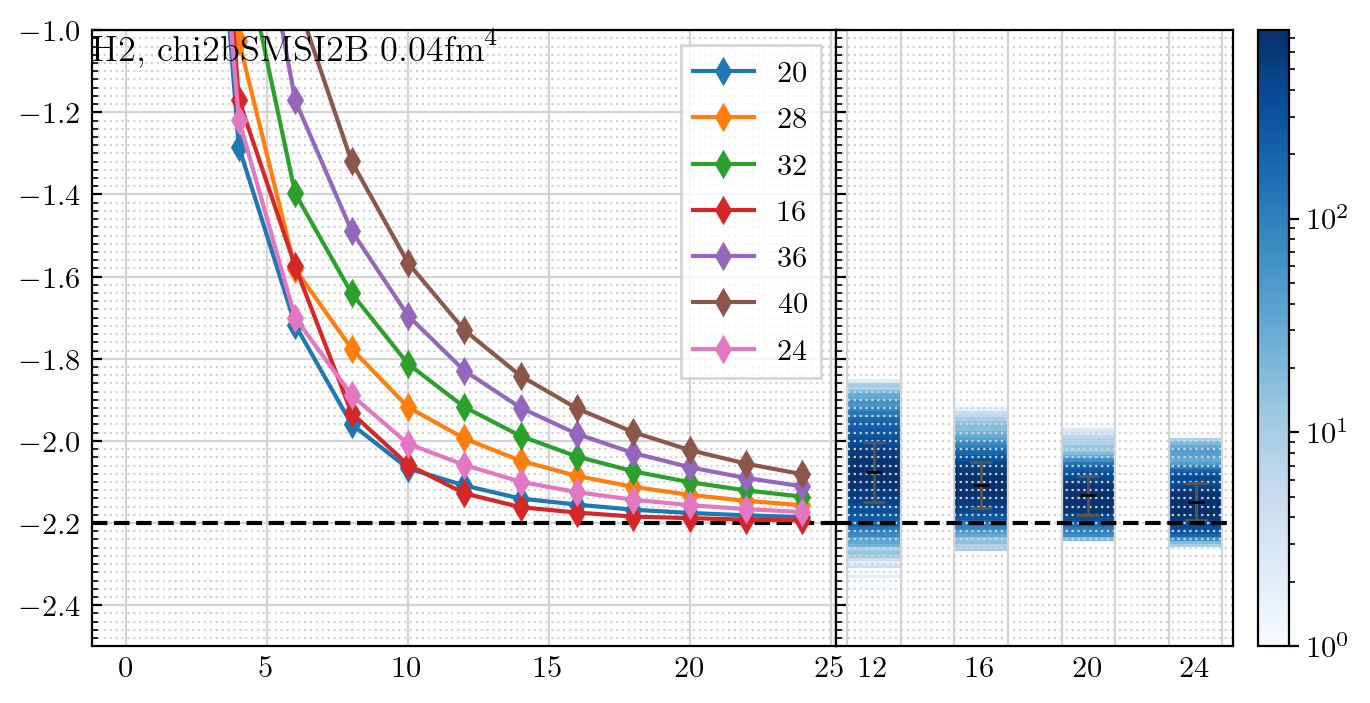
\includegraphics[]{media/example_evaluation.png}
  \caption{An example histogram of evaluations for the \textit{chi2bSMSI2B} interaction of \n{2}{H} using a SRG flow parmeter of \srg{0.04}. On the left side the raw NCSM calculations are shown to compare them to the extrapolation. On the right side, for each maximum $N_\mathrm{max}$, the histogramm as well as its mean and standard deviation is shown, which represent the extrapolated energy and its uncertainty.}
  \label{fig:example_evaluation}
\end{figure}
